% BESCHREIBUNG DER DOCUMENTCLASS
% a4paper 	-	weil wir ein Din-A4-Dokument benutzen.
% 12pt		-	Schriftgröße von 12 Punkt.
% listof=totoc 	-	heisst, dass das Tabellenverzeichnis (\listoftables) & das Abbildungsverzeichnis (\listoffigures) im Inhaltsverzeichnis aufgenommen werden.
% bibtotoc		-	Das Literaturverzeichnis wird ins Inhaltsverzeichnis aufgenommen.
% scrreprt		-	Das Template für diese Dokument ist ein KOMA-Script Report

\documentclass[a4paper, 12pt, hidelinks, listof=totoc, listoftables=totoc, bibliography=totoc]{scrreprt}

\usepackage{lmodern}									% Modernes Lateinisches Schriftbild benutzen
\usepackage[T1]{fontenc}								% Schriftbild glätten
\usepackage[utf8]{inputenc}								% UTF-8 als input encoding nutzen
\usepackage[ngerman]{babel}								% Deutsche Silbentrennung
\usepackage[babel, german=quotes]{csquotes}
\usepackage{xcolor}										% Damit man Farben benutzen kann
\usepackage{setspace}									%
\usepackage[a4paper]{geometry}							%
\geometry{left=25mm, right=25mm, top=25mm, bottom=25mm}	% Seitenränder setzen
\usepackage{titlesec}									%
\usepackage{graphicx}									%
\usepackage{graphics}									%
\usepackage{listings}
\usepackage{alltt}
\usepackage{nameref}\lstset{
  literate={ö}{{\"o}}1
           {ä}{{\"a}}1
           {ü}{{\"u}}1
           {Ö}{{\"O}}1
           {Ä}{{\"A}}1
           {Ü}{{\"U}}1
           {ß}{{\ss}}1
}
\usepackage{hyperref}									% für Hyperlinks
\usepackage{url}										% um lange URLs darzustellen
%\usepackage{amsmath}									% für mathematische Formeln
%\usepackage{subfigure}									% eine Möglichkeit, um Bilder nebeneinander zu plazieren
%\usepackage{subcaption}
\usepackage{subfig}										% um Bilder nebeneinander zu plazieren
\usepackage[font=footnotesize]{caption}					% nötig, um die Font-Größe für Captions festzulegen
\usepackage[export]{adjustbox}							% für Rahmen um figures
\usepackage[printonlyused]{acronym}									% Abkürzungsverzeichnis verwenden

\DeclareCaptionLabelFormat{andtable}{#1~#2  \&  \tablename~\thetable}	% für eine Caption für Abb. und Tab. nebeneinander

% Bibliographie mit biblatex/biber
\usepackage[backend=biber, style=alphabetic]{biblatex}
\addbibresource{biblio_scalajs.bib}


\graphicspath{{images/}}


%\definecolor{mid-red}{RGB}{224,0,0}
%\definecolor{mid-green}{RGB}{0,160,0}
%\definecolor{dark-blue}{RGB}{0,0,160}
\definecolor{mid-gray}{RGB}{127,127,127}
\definecolor{light-gray}{RGB}{244,244,244}
%\colorlet{keyword}{dark-blue}
%\colorlet{string}{mid-red}
%\colorlet{comment}{mid-green}
\colorlet{keyword}{black}
\colorlet{string}{black}
\colorlet{comment}{black}
\colorlet{linennumber}{mid-gray}
\colorlet{background}{light-gray}


% Sprachdefinitionen für Listings
\lstdefinelanguage{Scala}{
  morekeywords={
    abstract,case,catch,class,def,do,else,extends,false,final,finally,for,%
    forsome,if,implicit,import,lazy,match,mixin,new,null,object,override,%
    package,private,protected,requires,return,sealed,super,this,throw,trait,%
    true,try,type,val,var,while,with,yield%
  },
  otherkeywords={=>,<-,<\%,<:,>:,\#,@},
  sensitive=true,
  morecomment=[l]{//},
  morecomment=[s]{/*}{*/},
  morestring=[b]",
  morestring=[b]',
  morestring=[b]"""
}
\lstdefinelanguage{JavaScript}{
  morekeywords={
    break,case,class,catch,const,continue,debugger,default,delete,do,else,%
    export,extends,finally,for,function,if,import,in,instanceof,let,new,%
    return,super,switch,this,throw,try,typeof,var,void,while,with,yield%
    null,true,false,undefined,NaN%
  },
  sensitive=true,
  morecomment=[l]{//},
  morecomment=[s]{/*}{*/},
  morestring=[b]",
  morestring=[b]'
}
\lstdefinelanguage{HTML5}{
  language=html,
  tagstyle=\bfseries\color{keyword},
  morecomment=[s]{<!--}{-->},
  morestring=[b]",
  morestring=[b]'
}

% Styles für Listings
\lstdefinestyle{colored}{
  keywordstyle=\bfseries\color{keyword},
  commentstyle=\itshape\color{comment},
  stringstyle=\color{string}
}
\lstdefinestyle{uncolored}{
  keywordstyle=\bfseries,
  commentstyle=\itshape,
  stringstyle=\ttfamily
}
\lstdefinestyle{numbered}{
  numbers=left,
  numberstyle=\tiny\color{linennumber}
}
\lstdefinestyle{unnumbered}{
  numbers=none
}
\lstdefinestyle{framed}{
  backgroundcolor=\color{background}
}
\lstdefinestyle{unframed}{
  backgroundcolor=
}
\lstdefinestyle{basic}{
  basicstyle={\ttfamily\singlespacing\footnotesize}, 	% andere Font-Größen: \scriptsize \footnotesize \small
  showstringspaces=false,
  breaklines=true,
  breakatwhitespace=true,
  style=unnumbered,
  captionpos=b,
  %belowcaptionskip=4pt,
  literate={`}{{\`{}}}1			% for proper backticks
}
\lstdefinestyle{standard}{
  style=basic,
  style=colored,
  style=framed
}
\lstdefinestyle{standardnocol}{
  style=basic,
  style=uncolored,
  style=unframed,
  frame=single %, rulecolor=\color{mid-gray}
}
\lstdefinestyle{htmlnocol}{
  tagstyle=\bfseries
}
\lstdefinestyle{inline}{
  basicstyle={\ttfamily\small},
  breakatwhitespace=false
}
\lstdefinestyle{snippet}{
  aboveskip=-5pt,
  belowskip=0pt,
%    style=unframed,
    xleftmargin=10pt,
    frame=
}

% Default-Style für Listings. Kann überall im Text analog geändert werden.
\lstset{ style=standardnocol }

% Kurzbefehle für Inline-Code.
\newcommand{\code}[1]{\lstinline[language=Scala, style=inline]|#1|}
\newcommand{\scala}[1]{\lstinline[language=Scala, style=inline]|#1|}
\newcommand{\js}[1]{\lstinline[language=JavaScript, style=inline]|#1|}
\newcommand{\html}[1]{\lstinline[language=HTML5, style=inline]|#1|}

\newcommand{\TODO}[1]{\textcolor{red}{#1}\newline}
\newcommand{\TODOi}[1]{\textcolor{red}{\{#1\}}}
\newcommand{\REDOi}{\textcolor{red}{<- \{UMFORMULIEREN\}~}}


%Arial nutzen wer will...
%\renewcommand{\rmdefault}{phv} % Arial
%\renewcommand{\sfdefault}{phv} % Arial

% FORMATIERUNG DER ÜBERSCHRIFTEN ANFANG
	% Überschriftenformatierung
	% Erklärung: \titleformat{Überschriftenklasse}[Absatzformatierung]{Textformatierung}{Numerierung}{Abstand zwischen Numerierung und Überschrift}{Code davor}[Code danach]
	% 1. Ebene chapter
	\titleformat{\chapter}[hang]{\Large\bfseries}{\thechapter\quad}{0pt}{}
	% 2. Ebene -- section
	\titleformat{\section}[hang]{\large\bfseries}{\thesection\quad}{0pt}{}
	% 3. Ebene -- subsection
	\titleformat{\subsection}[hang]{\bfseries}{\thesubsection\quad}{0pt}{}
	% 4. Ebene -- subsubsection
	\titleformat{\subsubsection}[hang]{\bfseries}{\thesubsubsection\quad}{0pt}{}

	% Platz um die Überschriften
	% Erklärung: \titlespacing{Überschriftenklasse}{Linker Einzug}{Platz oberhalb}{Platz unterhalb}[rechter Einzug]
	\titlespacing{\chapter}{0pt}{0pt}{10pt}
	\titlespacing{\section}{0pt}{20pt}{10pt}
	\titlespacing{\subsection}{0pt}{20pt}{10pt}
% FORMATIERUNG DER ÜBERSCHRIFTEN ENDE

% FORMATIERUNG FÜR ZWISCHENÜBERSCHRIFTEN OHNE NUMERIERUNG
\newcommand{\MyMiniSec}[1]{\rmfamily\fontsize{12}{15}\selectfont
	\vspace{7pt}\textbf{#1} %\vspace{1.0cm}
}

% FORMATIERUNG FLIESSTEXT ANFANG
	% Absatzeinrueckung unterdruecken
	\setlength{\parindent}{0pt}
	% Abstand zwischen zwei Absaetzen setzen
	\setlength{\parskip}{6pt}
	% Zeilenabstand
	% Optionen: \singlespacing , \onehalfspacing , \doublespacing
	\onehalfspacing
% FORMATIERUNG FLIESSTEXT ENDE

% EIGENE KOPFZEILE ANFANG
	\usepackage{scrpage2}
	\clearscrheadfoot
	\ihead[\footnotesize{\textnormal{\headmark}}]{\footnotesize{\textnormal{\headmark}}}
	\ohead[\footnotesize{\pagemark}]{\footnotesize{\pagemark}}
	\automark{chapter}
	% Numerierung nur bis subsection
	\setcounter{secnumdepth}{2}
% EIGENE KOPFZEILE ENDE


% Wird gebraucht für die Titelseite...
\newcommand{\RM}[1]{\MakeUppercase{\romannumeral #1{}}}

% Erstellung eines Index
\makeindex

%%%%%%%%%%%%%%%%%%%%%%%%%%%%%%%%%%%%%%%%%%%%%%%%%%%%%%%%
% BEGIN DOCUMENT // HIER FÄNGT DER INHALT AN
%%%%%%%%%%%%%%%%%%%%%%%%%%%%%%%%%%%%%%%%%%%%%%%%%%%%%%%%
\begin{document}

\begin{titlepage}
\begin{center}
	\begin{figure}[!h]
		
\includegraphics[scale=1]{./title/Beuth_Logo_horizontal.jpg}
	\end{figure}

	% vertikaler Zwischenraum
	\vspace{15mm}

	\large
		\textbf{Fachbereich \RM{6} $\cdot$ Informatik und Medien\\[3mm]
		Studiengang Medieninformatik}\\

	\vspace{15mm}

	\Large
		\textbf{Bachelorarbeit}\\[5mm]
	\normalsize
		zur Erlangung des akademischen Grades\\
		Bachelor of Science (B.Sc.)\\

	\vspace{15mm}

	\huge
		\textbf{Evaluierung von Scala.js \\
		für interaktive Weboberflächen }\\ [0,5cm]
	
	\Large
		\textbf{Untertitel ... TODO}\\[2cm]

	\normalsize
	\begin{tabular}{rl}
		vorgelegt von: & Sebastian Dassé \\
		Matrikelnummer: & 791537 \\
		am: & \today \\
		& \\
		Betreuer: & Prof. Christoph Knabe\\
		Gutacher: & Prof. Dr. Elmar Böhler\\
	\end{tabular}\\
\end{center}
\end{titlepage} % Import der Titelseite aus dem Ordner "title".

%\pagenumbering{gobble} % Keine Seitennumerierung

\pagestyle{empty} % Keine Kopfzeile


% % % % % % % % % % % % % % % % % % % % % % % % % % % % % % % %
%\begin{abstract}
%
%\Large
%	\textbf{Abstract}
%
%\normalsize
%
%
%ping
%
%pang
%
%pong \\
%
%
%ping
%
%pang
%
%pong
%\end{abstract}


\pagestyle{scrheadings} % Kopfzeile an

\pagenumbering{roman}



% % % % % % % % % % % % % % % % % % % % % % % % % % % % % % % %
\tableofcontents

\newpage

\pagenumbering{arabic}


% % % % % % % % % % % % % % % % % % % % % % % % % % % % % % % %
\chapter{Einleitung}

%TODO Zitate checken, ggf. ergänzen um "`vgl."'

Von modernen Weboberflächen wird Interaktivität in einem Maße erwartet, wie es noch vor wenigen Jahren ausgewachsenen Desktopanwendungen vorbehalten war. Klassische Webseiten sind echten Web-Anwendungen (\emph{Rich Internet Applications}) gewichen und die Zahl an Anwendungen, die als Online-Dienst in der "`Cloud"' angeboten werden (\emph{Software as a Service}), steigt. Und die Tatsache, dass ein einfacher Aufruf im Browser an die Stelle einer oft als mühsam empfundenen Installation auf dem Desktop tritt, macht Web-Anwendungen aus Nutzersicht äußerst attraktiv.

%steigen auch die Erwartungen der Web-Anwender Interaktion selbstverständlich

Um Interaktivität im Browser zu ermöglichen, reicht HTML\footnote{\ac{HTML}} allein nicht aus. Eine zusätzliche Technologie ist nötig: JavaScript. Moderne Browser enthalten deshalb eine JavaScipt-Engine, mit deren Hilfe JavaScipt-Programme ausgeführt werden können. Daneben existieren zwar auch Plugin-basierte Alternativen (Flash, Java Applets, MS Silverlight), doch diese verlieren rapide an Bedeutung, unter anderem durch die verbesserte Browser-Unter-stützung für den neuen HTML5-Standard. JavaScript dominiert hier bei weitem und kann als De-facto-Standard betrachtet werden\footnote{90 \% aller Websites verwenden aktuell JavaScript. \cite{w3techs.CLI}}.


\section{Motivation}

JavaScript wurde 1995 von Brendan Eich für Netscape innerhalb von zehn Tagen entwickelt.\footnote{Es ging damals darum, den Konkurrenten Java auszustechen: "`JS had to ,look like Java` only less so, be Java's dumb kid brother or boy-hostage sidekick. Plus, I (sic!) had to be done in ten days or something worse than JS would have happened."' \cite{eich2010.KBE}}  Der Einsatzzweck der Sprache bestand zu dieser Zeit in erster Linie darin, statische Webseiten durch interaktive Elemente attraktiver zu machen. Komplexe clientseitige Web-Anwendungen, wie sie heute mit JavaScript entwickelt werden, hatte man damals nicht im Blick. Um der wachsenden Komplexität der Web-Anwendungen gerecht zu werden, kommt eine immer breiter werdende Palette an JavaScript-Frameworks zum Einsatz, durch die auf strukturierende Hilfsmittel und auf erweiterte Standardfunktionalitäten zurückgegriffen werden kann. Diese erleichtern zwar die Arbeit und führen schneller zu qualitativ hochwertigerer Software, die Einarbeitung in jedes dieser unterschiedlichen Frameworks verlangt allerdings einen erheblichen Aufwand.

Die Sprache JavaScript ist aus verschiedenen Gründen problematisch. So existieren zahlreiche Inkonsistenzen und kontraintuitive Sprachbesonderheiten, welche zwar dokumentiert sind, aber das Programmieren erschweren. JavaScript ist dynamisch typisiert, was besonders in größeren Projekten zum Problem wird. Refactorings sind schwierig und es kann zu schwer zu findenden Laufzeitfehlern kommen (mit Meldungen wie dem notorischen "`undefined is not a function"'). Zusätzlich sind viele Konzepte, wie zum Beispiel Klassen, Modularisierung oder Konstanten, in JavaScript unspezifiziert. Sie sind zwar umsetzbar, doch häufig existieren viele verschiedene Wege um zu erreichen, was in anderen Programmiersprachen einfach Teil der Sprache ist. 
Das führt dazu, dass für solche Standardprobleme entweder das "`Rad neu erfunden"' wird, oder doch jedes Mal neu auszuhandeln ist, welcher Weg beschritten werden soll. Häufig bieten hier Frameworks oder Librarys\footnote{Programmbibliotheken} von Drittanbietern Lösungen. Allerdings um den Preis zusätzlicher Lernzeit.

% siehe jeweils Einleitung von Doeraene 2013 und Haoyi 2015

Hier setzen nun verschiedene Projekte an, die es erlauben, in einer konsistenteren und bequemeren Sprache zu programmieren, um den Code schließlich nach JavaScript zu kompilieren, das heißt: automatisch zu übersetzen. Dabei wird JavaScript als Plattform betrachtet, oder auch als "`Assemblersprache des Webs"' \cite{meijer2011.JLA}. Viele dieser transkompilierenden Sprachen bieten dabei eine statische Typisierung. Sébastien Doeraene, Kopf des Scala.js-Projekts, kritisiert allerdings diese bisherigen Versuche als unzulänglich. Dabei macht er zwei vollkommen unterschiedliche Ansätze aus. Dem einen Ansatz, bei dem von \mbox{JavaScript} ausgegangen und dieses um \emph{syntaktischen Zucker}\footnote{engl. \emph{syntactic sugar}, Syntaxerweiterungen zur Vereinfachung der Schreibweise} (CoffeeScript) oder ein Typsystem (TypeScript) erweitert wird, attestiert er zwar einen gewissen Nutzen, moniert aber, dass die Sprache dadurch nur wenig an Ausdruckskraft gewinnt. Bei der anderen Gruppe, handelt es sich um völlig neue (Dart) oder schon existierende Sprachen (Java mit GWT). Diese Sprachen erlauben zwar ein höheres Abstraktionslevel und vermeiden alle Probleme von JavaScript, doch mangelt es ihnen an echter Interoperabilität mit \mbox{JavaScript}, was insbesondere die Interaktion mit dem \ac{DOM}, aber auch mit JavaScript-Librarys erschwert oder sogar unmöglich macht. Der Grund hierfür liegt darin, dass JavaScript-Werte nicht in das strengere Typsystem überführt werden können und daher keine \emph{First-Class-Citizens} der Sprache sind. \cite[S. 1]{doeraene2013.TDI}

Ein weiteres großes Problem der Web-Entwicklung stellt traditionell die Schnittstelle zwischen Client und Server dar. Hier existiert eine Sprachgrenze, wobei auf Serverseite verschiedene Sprachen im Einsatz sind (hier dominiert PHP, gefolgt von unter anderem Java \cite{w3techs.SRV}). Die Wiederverwendung von Code über diese Grenze hinweg ist nicht möglich, weshalb Algorithmen mehrfach implementiert werden müssen, oder mühsam durch Ajax-Aufrufe an einem Ort gehalten werden. Auch die Einhaltung gemeinsamer Schnittstellen ist dadurch schwierig und fehlerträchtig. Eine Sprache für beide Seiten, Client und Server, ist demnach wünschenswert, würde sie doch genau dies erlauben: die Wiederverwendbarkeit von Code und die Definition gemeinsamer Schnittstellen. \cite[\#SharingCode]{haoyi.HOS}

Mit Node.js existiert seit einigen Jahren auch eine serverseitige JavaScript-Laufzeitumge-bung\footnote{Node.js basiert auf der V8 JavaScript Engine. Es arbeitet eventgesteuert, asynchron und kennt keine Threads. \url{https://nodejs.org/}}, so dass Einsprachigkeit erreichbar ist. Allerdings mit allen beschriebenen Nachteilen der Sprache JavaScript.

Scala.js verspricht Lösungen für die angesprochenen Probleme. Scala wird als Quellsprache verwendet und nach JavaScript übersetzt. Damit stehen dem Programmierer die mächtigen Sprachmittel von Scala zur Verfügung: ein konsistentes statisches Typsystem, eine prägnante Syntax, ausdrucksstarke Konstrukte (wie \emph{Pattern Matching} und \emph{For-Comprehensions}) und eine umfangreiche Collections-Library. Gleichzeitig soll eine sehr gute Interoperabilität mit JavaScript möglich sein.


\section{Zielstellung}

Mit dem Fokus auf der Entwicklung von interaktiven Weboberflächen soll in dieser Arbeit untersucht werden, ob und inwiefern dieses Versprechen eingehalten wird und wie gut Scala.js zur Entwicklung von Weboberflächen geeignet ist. Dazu soll erforscht werden, welcher Gewinn sich aus dem Einsatz von Scala.js ziehen lässt, aber gegebenenfalls auch, welche besonderen Schwierigkeiten sich hierbei ergeben.

Hierfür sind verschiedene Fragen zu klären. Es gilt, die grundlegenden Mechanismen dieses Werkzeugs zu erproben und den Konfigurationsaufwand einzuschätzen. Dann soll Klarheit darüber gewonnen werden, wie sich häufige Anforderungen aus dem Bereich der Web-Entwicklung mit Scala.js umsetzen lassen und ob der Entwickler hierbei an Grenzen stößt. Als wichtiger Punkt soll auch betrachtet werden, welche Auswirkungen die Verwendung von Scala.js auf die Code-Qualität\footnote{Dieser Begriff wird in Kapitel \ref{chap:methods} eingegrenzt.} hat. Aber auch der Komfort des Arbeitens mit Scala.js soll untersucht werden, etwa mit welcher Schnelligkeit entwickelt werden kann. Außerdem ist die Frage wichtig, ob Scala.js-Anwendungen mit solchen, die auf herkömmliche Weise in JavaScript entwickelt wurden, mithalten kann.

Um diesen Fragen nachzugehen, werden in einigen Fallstudien verschiedene kleinere Beispielprogramme besprochen. Basierend auf diesen Erfahrungen soll die Nützlichkeit und Einsatzfähigkeit von Scala.js eingeschätzt werden.


\section{Abgrenzung}

Einige Probleme können in dieser Arbeit nicht behandelt werden. Dazu zählt als erstes die Kompatibilität von Webseiten mit älteren Browsern. \TODOi{Ebenfalls nicht diskutiert wird die Frage, ob \ac{HTML}-Dokumente besser auf Client- oder Serverseite generiert werden sollten. In einem praktischen Client-Server-Beispiel wird die Serverseite bewusst einfach gehalten. Insbesondere wird auf den Einsatz einer Datenbank verzichtet und die Themen Authentifizierung und Sitzungsverwaltung bewusst ausgeblendet. (???)}


\section{Aufbau der Arbeit}

Kapitel \ref{chap:basics} stellt das technische Umfeld vor und klärt in diesem Zusammenhang wichtige Grundbegriffe. Insbesondere werden hier die Gemeinsamkeiten und Unterschiede der Programmiersprachen Scala und JavaScript verdeutlicht.

Kapitel \ref{chap:scala.js} liefert einen Überblick über Scala.js. Dazu werden zunächst die konzeptionellen Grundlagen erklärt. Danach wird auf einige semantische Abweichungen von Scala eingegangen und die Interoperabilität mit JavaScript erläutert. Schließlich wird das technische Ökosystem beschrieben, das Scala.js bietet.

Kapitel \ref{chap:methods} erläutert die Vorgehensweise bei der Untersuchung und stellt dafür Kriterien auf.

Kapitel \ref{chap:setup} enthält eine Anleitung zur Installation der benötigten Software und erklärt die nötigen Schritte um die Fallbeispiele zur Ausführung zu bringen.

Kapitel \ref{chap:case-studies} stellt einige abgegrenzte Fallstudien vor, in denen anhand praktisch umgesetzter Beispielimplementierungen wichtige Aspekte von Scala.js untersucht und eingeschätzt werden.

In Kapitel \ref{chap:conclusion} werden die Ergebnisse der Arbeit zusammengefasst und ausgewertet. Schließlich wird ein kurzer Ausblick auf die Zukunft von Scala.js gegeben.


\section{Anmerkung zur Zitierweise}

Um die Fundstellen in Internetquellen präziser zu bezeichnen, wird in geeigneten Fällen statt einer Seitenzahl die Sprungmarke im \ac{HTML}-Dokument, erkennbar am vorangestellten \code{\#} verwendet. Diese muss in der Adresszeile des Browsers lediglich an die URL\footnote{\ac{URL}} angehängt werden. Für Videoquellen wird eine Zeitangabe in Minuten gemacht.


% % % % % % % % % % % % % % % % % % % % % % % % % % % % % % % %
\chapter{Technisches Umfeld und Grundbegriffe}\label{chap:basics}

Der hauptsächliche Zweck von Scala.js besteht darin, bestimmten Mängeln der Sprache JavaScript dadurch zu begegnen, dass sie als eine Ziel-Plattform der Sprache Scala betrachtet wird. Für ein besseres Verständnis sollen hier deshalb zunächst beide Sprachen, Scala und JavaScript, besprochen werden. Im Anschluss folgt zur besseren Einordnung ein knapper Überblick über die Web-Kerntechnologien \ac{HTML} und \ac{CSS} und sowie eine kurze Vorstellung des Buildtools sbt.

\section{Scala}

Scala ist eine moderne Multiparadigmen-Programmiersprache, die objektorientierte und funktionale Programmierkonzepte mit einer statischen Typisierung verbindet. Sie wird seit 2001 federführend von Martin Odersky an der \ac{EPFL} entwickelt. Erstmals öffentlich vorgestellt wurde die Sprache 2004 mit den Worten: "`Scala [...] is designed to express common programming patterns in a concise, elegant, and type-safe way."' \cite{schinz2004.ASP} Seit der Gründung der Firma Typesafe 2011 durch Odersky und Jonas Bonér\footnote{Bonér ist der Autor von \emph{Akka}, einem Toolkit und einer Laufzeitumgebung zur Entwicklung fehlertoleranter nebenläufiger und verteilter Anwendungen. Es basiert auf einem Modell, bei dem \emph{Aktoren} genannte nebenläufige Einheiten durch Nachrichtenaustausch miteinander kommunizieren. Akka ist Teil der Typesafe-Plattform. \url{http://akka.io/}} erfährt die Entwicklung von Scala als Teil der \emph{Typesafe Reactive Platform} nun auch kommerzielle Unterstützung.
Hier wird unter anderem die IDE\footnote{Integrierte Entwicklungsumgebung, engl. \ac{IDE}}-Integration für Scala vorangetrieben und das Buildtool \emph{sbt} entwickelt. \cite{scala-lang2011.CSS} 

Scala verwendet eine prägnante, schlanke Syntax. So lässt sich zum Beispiel eine einfache Klasse sehr kompakt schreiben: \scala{class Foo(val bar: Int)}. Damit sind sowohl ein Konstruktor als auch die Instanzvariable (\scala{bar}) definiert. Durch diese Prägnanz sind Scala-Programme eher kurz. Ein Java-Programm lässt sich in Scala mit etwa der halben Anzahl an \emph{Lines of Code}\footnote{engl. für "`Code-Zeilen"', eine Softwaremetrik. Im einfachsten Fall die tatsächliche Anzahl aller Zeilen aus denen die Quelldateien bestehen. Es existieren aber verschiedene Zählweisen, wie die ohne Leer- und Kommentarzeilen.} formulieren. Das reduziert den Schreib- und Leseaufwand und die Gelegenheit Fehler zu machen.

Scala erlaubt es, auf einem relativ hohen Abstraktionslevel zu programmieren und erleichtert so den Umgang auch mit komplexen Systemen.

Scala-Programme kompilieren zu Java-Bytecode und laufen auf der \ac{JVM}. Ihre Performance ist mit der von Java-Programmen vergleichbar. Scala-Code kann Java-Code aufrufen. Dadurch hat der Scala-Programmierer\footnote{Genderklausel: Der Einfachheit halber wird im Text die männliche Form verwendet. Natürlich ist auch die Programmiererin gemeint.} automatisch auch alle Java-Librarys zur Verfügung. Scala-Code kann auch von Java-Code aufgerufen werden, aber hier sind manchmal einige Feinheiten zu beachten. \cite[S. 13 ff.]{odersky2008.PIS}

Der Einstieg in die Sprache Scala ist relativ einfach. Durch die Mächtigkeit der Sprachmittel und die Vielzahl der sich daraus ergebenden Möglichkeiten, ist für ein tieferes Verständnis allerdings ein hoher Lernaufwand nötig.

%(>>Wurzeln: Syntax ähnlich Java, ML)


\subsection{Objektorientierung}

Scala ist eine rein objektorientierte Sprache: Jeder Wert ist ein Objekt. Das schließt auch numerische Werte und Funktionen ein, primitive Typen wie in Java existieren nicht. Doch die Objektorientierung geht sogar noch weiter: In Scala ist jede Operation ein Methodenaufruf. So ist \scala{1 + 2} der Aufruf der Methode \scala{+} an einer Instanz der Klasse \scala{Int} und könnte auch als \scala{1.+(2)} ausgedrückt werden. Konsequenterweise sind auch statische Methoden unbekannt. Stattdessen werden mit dem Schlüsselwort \scala{object} Singleton-Objekte definiert, die Methoden und Werte aufnehmen können, welche nicht Attribute der Instanz einer Klasse sind. Diese können entweder alleinstehend sein oder als sogenanntes Begleitobjekt (\emph{companion object}) einer gleichnamigen Klasse auftreten.

Benutzerdefinierte Typen lassen sich mithilfe von Klassen und \emph{Traits} definieren. Traits sind den Interfaces in Java ähnlich, sie können allerdings Implementierungen von Methoden und sogar Felder enthalten. Außerdem können Traits mehrfach beerbt werden (man spricht hierbei auch von \emph{mixin class composition}).

Die Modularisierung von Programmen funktioniert grundsätzlich ähnlich wie in Java, allerdings stellt Scala flexiblere und generischere Mittel zur Verfügung. Importe können grundstäzlich überall platziert werden. Dabei können neben Paketen und Paket-Membern auch Objekte importiert werden. Member können auch unter anderem Namen importiert werden, sei es um Namenskonflikte zu vermeiden oder um häufig verwendete Namen abzukürzen.
Pakete können, anders als in Java, beliebig verschachtelt werden. Die Zugriffsmodifizierer werden konsistenter und granularer als in Java gehandhabt. Beginnt etwa die Deklaration einer Methode mit \scala{private[this]}, so darf nur durch das Objekt selbst auf diese Methode zugegriffen werden. \cite[S. 9 f., S. 233 ff.]{odersky2008.PIS}\cite{scala-lang.ATS}

\subsection{Funktionale Programmierung}

%funktional (aber auch imperativ)

%Scala unterstützt funktionale Programmierung.
Scala ist eine vollständig funktionale Sprache\footnote{Funktionale Programmierung basiert auf dem in den 1930er Jahren von Alonzo Church entwickelten Lambda-Kalkül. Dessen zentrale Idee besteht darin, dass Funktionen anonym definiert werden. Das Lambda-Kalkül ist Turing-vollständig, und somit gleich mächtig wie imperative Sprachen. Jedes imperative Programmierkonstrukt lässt sich demnach auch funktional ausdrücken.}. Funktionen sind in Scala First-Class-Citizens, das heißt sie haben denselben Status wie alle anderen Daten. Sie können einer anderen Funktion als Parameter übergeben werden oder von einer anderen Funktion zurückgegeben werden. Diese "`andere"' Funktion bezeichnet man als Funktion höherer Ordnung. Funktionen können ineinander verschachtelt werden und anonym als \emph{Funktionsliterale} verwendet werden.

Funktionen bilden Eingabewerte auf Ausgabewerte ab, ohne dabei den Zustand der Eingabewerte zu verändern. Man sagt: Sie sind frei von Nebenwirkungen (\emph{side effects}). Zusätzlich sind Funktionen referentiell transparent, das heißt sie liefern für gleiche Argumente immer das gleiche Ergebnis. Für jeden Eingabewert kann der Funktionsaufruf durch sein Resultat ersetzt werden, ohne dass sich dadurch die Semantik ändert. Durch diese Eigenschaften wird die funktionale Programmierung zunehmend attraktiv für den Einsatz in nebenläufigen Programmen. Einfach ausgedrückt: Werte die sich nie ändern müssen auch nicht synchronisiert werden.

Darüberhinaus kennt Scala \emph{Closures}, \emph{Currying} und \emph{For-Comprehensions}.

Scala unterstützt zwar die nebenwirkungsfreie funktionale Programmierung mit unveränderlichen (\emph{immutable}) Daten, lässt einem aber die Wahl, gegebenenfalls im imperativen Stil zu programmieren. \cite[S. 6 ff.]{piepmeyer2010.GFP}\cite[S. 10 ff.]{odersky2008.PIS}

\subsection{Einheitliches statisches Typsystem}\label{subsec:scala-types}

Scala verfügt über ein ausdrucksstarkes einheitlich Typsystem mit einer gemeinsamen Superklasse \scala{Any} von der jede Klasse erbt. \scala{Any} hat exakt zwei direkte Subklassen: \scala{AnyVal} und \scala{AnyRef}. 

Von \scala{AnyVal} erben die neun Scala-eigene Werteklassen: \scala{Byte}, \scala{Short}, \scala{Char}, \scala{Int}, \scala{Long}, \scala{Float}, \scala{Double} und \scala{Boolean}, die den primitiven Typen in Java entsprechen\footnote{sie werden sogar zur Laufzeit durch primitive Java-Typen ersetzt} und \scala{Unit}, das etwa \scala{void} in Java entspricht. \scala{AnyRef}, die andere Subklasse von \scala{Any}, ist die Basisklasse für alle Referenzklassen. Auf der Java-Plattform ist \scala{AnyRef} nur ein Alias für die Klasse \mbox{\scala{java.lang.Object}}.

Außerdem existieren noch zwei spezielle Klassen: \scala{Null} und \scala{Nothing}. \scala{Nothing} ist eine gemeinsame Subklasse jeder anderen Klasse. Dieser Typ kann keine Werte enthalten, wird aber benötigt um zum Beispiel den Typ der leeren Liste zu definieren: \mbox{\scala{List[Nothing]}}. Die Klasse \scala{Null} enthält \scala{null} als einzigen Wert und ist der Subtyp aller Referenzklassen, also all der Klassen, die von \scala{AnyRef} erben.

Scala ist statisch typisiert, das bedeutet es findet eine Typprüfung zur Compile-Zeit statt. Daraus leiten sich sich verschiedene entscheidende vorteilhafte Eigenschaften ab. Ein Typ ist nichts anderes als die Festlegung des Wertebereichs und der möglichen Operationen für ein Objekt. Ist der Typ eines Objekts bekannt, so werden an ihm beispielsweise nie Methoden aufgerufen oder auf Attribute zugegriffen werden können, die er nicht besitzt. Solche Programmierfehler würde der Compiler melden und das Programm einfach nicht übersetzen. Mit der statischen Typprüfung sind demnach echte Garantien verbunden, die bestimmte Laufzeitfehler sicher ausschliessen, und zwar sicherer als jeder Unit-Test.

Diese Typsicherheit bedeutet auch eine größere Sicherheit beim Refactoring und eine deutlich stärkere Unterstützung durch IDEs: beim Refactoring, bei der komfortablen Quellcode-Navigation (wie etwa das Springen zur Definition eines Werts) und durch typbasierte automatische Code-Vervollständigung. Nicht zuletzt ist Code automatisch besser dokumentiert, wenn die Typen der Attribute, Parameter und Funktionsrückgabewerte bekannt sind.

Trotz strenger Typisierung erlaubt Scala einen flexiblen Umgang mit seinen Typen. Durch ein System der automatischen Typableitung (\emph{Typinferenz}) werden redundante Typangaben vermieden. Häufig kommen Deklarationen sogar ganz ohne explizite Typangaben aus. Zusätzlich erlaubt der eingebaute Mechanismus des Pattern Matching\footnote{raffinierte Form einer \code{switch}-Anweisung anhand der Struktur oder dem Typ eines Objekts} einen sehr flexiblen Umgang mit streng getypten Werten.

Scala erlaubt generische Klassen, innere Klassen, abstrakte Typen als Member, zusammengesetzte Typen (\emph{compound types}) und implizite Parameter. \cite[S. 16 ff., S. 205 ff.]{odersky2008.PIS}\cite[S. 113 ff.]{piepmeyer2010.GFP}\cite{scala-lang2011.CSS}

\subsection{Erweiterbarkeit}

Scala trägt die Erweiterbarkeit im Namen ("`scalable language"').
%"eine Sprache die mitwächst" ("a language that grows on you")
Die Sprache hat einen relativ kompakten Kern und liefert einen großen Umfang an Funktionalität in Form einer Standardbibliothek. Diese enthält unter anderem ein äußerst unfangreiches Collections-Framework, eine Mathematik-Bibliothek, Bibliotheken für reguläre Ausdrücke, zur XML\footnote{\ac{XML}}-Manipulation, zur nebenläufigen Programmierung mit \emph{Futures} und \emph{Promises} und eine \emph{Aktoren}-Bibliothek, welche Nebenläufigkeit durch Nachrichtenaustausch realisiert.\footnote{Einen guten Überblick über die Standardbibliothek bietet die Dokumentation: \url{http://www.scala-lang.org/api/current/\#package}} Die Sprache stellt auch mächtige Mittel zur Verfügung, um flexible Librarys und DSL\footnote{Domänenenspezifische Sprache, engl. \ac{DSL}}s zu entwickeln. Zum Beispiel kann die Vererbung durch die Kombination beliebig vieler Traits sehr flexibel gehandhabt werden. Es ist ferner möglich, implizite Konvertierungen zu definieren. Die Infix- und Postfix-Notation in Verbindung mit der erlaubten Verwendung von Sonderzeichen für Methodennamen erlaubt es, eigene Operatoren zu schreiben \linebreak(\mbox{\scala{1 + 2}} ist die Infix-Notation für \scala{1.+(2)}). Es ist sogar möglich eigene Kontrollstrukturen zu erzeugen, indem man Methoden mit Operationen parametrisiert\footnote{durch \emph{by-name evaluation}}. \cite[S. 4 ff.]{odersky2008.PIS}

\subsection{Tools und Ökosystem}

Scala wird mit einem sehr nützlichen interaktiven Kommandozeilen-Interpreter ausgeliefert (auch: \ac{REPL}). Zur IDE-Integration existieren Plugins für Eclipse\footnote{Es existiert auch eine komplette Eclipse-basierte Scala IDE.}, IntelliJ IDEA und NetBeans. Für Tests eignet sich ScalaTest, das viele unterschiedliche Teststile unterstützt. Auch die in der Java-Welt etablierten Frameworks JUnit und TestNG können verwendet werden. Mit \emph{sbt} existiert ein Buildtool, das für Scala-Projekte der De-facto-Standard ist. Aber auch mit Ant und Maven sind Builds möglich. Auf der Scala-Website\footnote{\url{http://docs.scala-lang.org/}} finden sich neben der Dokumentation der API\footnote{Programmierschnittstelle, engl. \ac{API}} auch offizielle Tutorials und ein Style Guide.



\section{JavaScript}

JavaScript ist eine dynamische Skriptsprache, die es erlaubt, objektorientiert und funktional zu programmieren. Der primäre Zweck von JavaScript ist es, aus statischen Webseiten interaktive Webanwendungen zu machen \cite[S. 361]{flanagan2011.JDG}.

Die wichtigste Zielplattform für JavaScript ist der Browser. Dieser benötigt zur Ausführung von JavaScript eine JavaScript-Engine, die den Code zur Laufzeit interpretiert und in Maschinencode übersetzt. Aus Performancegründen sind moderne JavaScript-Engines allerdings meistens keine Interpreter mehr, sondern führen eine Just-in-time-Kompilierung (JIT)\footnote{\url{https://en.wikipedia.org/wiki/Just-in-time_compilation}} durch. Einige aktuell verbreitete JavaScript-Engines sind V8 (Google Chrome und Opera), SpiderMonkey (Mozilla Firefox) und Nitro (Apple Safari). Darüber hinaus ist in den letzten Jahren auf der Serverseite Node.js (V8) als leichtgewichtige JavaScript-Laufzeitumgebung populär geworden.

JavaScript wird unter dem offiziellen Namen ECMAScript von der Organisation Ecma International standardisiert (als Standard ECMA-262). Der aktuell von allen wichtigen Browsern unterstützte Standard ECMAScript 5.1 stammt aus dem Jahr 2011\footnote{\url{http://www.ecma-international.org/ecma-262/5.1/}}. Die im Juni 2015 veröffentlichte Version ECMAScript 6 enthält viele Verbesserungen um die Sprache zu modernisieren\footnote{\url{http://www.ecma-international.org/publications/standards/Ecma-262.htm}}, ist aber momentan noch nicht ausreichend in den verbreiteten Browsern implementiert.

JavaScript ähnelt zwar in der Syntax seinem ungleichen Namensvetters Java, die Semantik unterscheidet sich hingegen teilweise stark \cite{eich1996.JSL}.


\subsection{Objektorientierung}\label{subsec:js-oo}

JavaScript ist eine objektorientierte Sprache. Objekte auf können auf drei Arten erzeugt werden:

\begin{itemize}
  \item als Literal: \js{var foo = \{bar: 123\}}
  \item mit \js{new} gefolgt vom Aufruf einer Konstruktor-\code{Function}
  \item mit \js{Object.create()}, wobei als Parameter der Konstruktor übergeben werden muss.
\end{itemize}

Objekte haben Eigenschaften (\emph{Propertys}), die primitive Werte, Referenzen auf andere Objekte, oder Methoden sein können. Propertys eines Objekts können neben der geläufigen Punkt-Notation (\js{foo.bar}) auch durch den in eckigen Klammern eingeschlossene Membernamen als String \mbox{(\js{foo["bar"]})} referenziert werden. Bei JavaScript-Objekten handelt es sich nämlich im Grunde um Collections benannter Werte, das heißt sie sind nichts anderes als assoziative Arrays\footnote{eine Collection, die aus Schlüssel-Wert-Paaren besteht, in Scala: \emph{Map}, in anderen Sprachen gelegentlich auch: \emph{Dictionary}}. Daher werden bei Bedarf Objekte auch explizit als Collections verwendet, wobei als Schlüssel allerdings nur Strings erlaubt sind.

Das Konzept von Klassen ist nicht Teil der Sprache. Vererbung funktioniert in JavaScript über den Prototypen. Dazu referenziert jedes JavaScript-Objekt ein anderes Objekt, deren Eigenschaften es erbt: den Prototypen. Objekte die vom selbem Prototypen erben, kann man als Klasse auffassen. \cite{mdn.WWO}\cite[S. 115 ff., S. 199 ff.]{flanagan2011.JDG}

\subsection{Funktionale Programmierung}

Funktionen sind in JavaScript First-Class-Citizens (wie in Scala). Sie können in Variablen gespeichert oder verschachtelt werden, können als Parameter übergeben werden oder als Rückgabewert einer Funktion dienen. Damit sind auch Funktionen höherer Ordnung möglich. Häufige Anwendungsfall für Funktionen höherer Ordnung in JavaScript sind sogenannte Callback-Funktionen und Closures\footnote{anonyme Funktionen mit Zugriff auf ihren Erstellungskontext}. Durch \emph{Currying} lässt sich auch die partielle Anwendungen von Fuktionen umsetzen. --- All dies ist aber im Vergleich zu Scala mühsamer und \emph{verbose} (wortreich).

Die Behandlung von Funktionsparametern ist in JavaScript äußerst flexibel. Werden beim Funktionsaufruf weniger Parameter übergeben als im Methodenheader deklariert sind, erhalten diese automatisch den Wert \js{undefined}. Werden zu viele Parameter übergeben, so werden diese einfach ingoriert. Auf alle tatsächlich übergebenen Argumente kann innerhalb einer \js{Function} durch eine Liste namens \js{arguments} zugegriffen werden, unabhängig von im Methodenheader deklarierten Parametern.

\subsection{Dynamische Typisierung}

JavaScript ist eine in äußerstem Maße dynamische Sprache. Objekte können in JavaScript zur Laufzeit grundlegend verändert werden. Methoden können hinzugefügt, Methoden zu Attributen gemacht oder durch andere Methoden ersetzt werden.

Variablen sind in JavaScript nicht typisiert. Daher ist es zulässig, einer Variablen erst einen Wert vom Typ A und später einen Wert vom Typ B zuzuweisen. Außerdem finden in JavaScript viele implizite Konvertierungen statt, wenn in einem Programm ein anderer als der erwartete Typ verwendet wird, zum Beispiel von \js{Number} nach \js{String} oder von einem beliebigen Typ nach \js{Boolean}.

JavaScript unterscheidet nur wenige Datentypen. Es gibt die primitiven Typen: \js{Boolean}, \js{Number} und \js{String}. 
Dabei werden alle Zahlen ohne Unterscheidung zwischen Ganz- und Fließpunktkommazahlen als \js{Float} repräsentiert. Alle primitiven Typen sind \emph{immutable}. Außerdem werden sie ausnahmslos als Objekte behandelt. Dazu existieren Wrapper, in welche die primitiven Typen bei Bedarf automatisch konvertiert werden. Auf diese Weise können beispielsweise Methoden der Wrapper-Klasse \js{String} direkt an einem Stringliteral aufgerufen werden (\js{\"foo\".toUpperCase()}).

Daneben existieren zwei spezielle Werte: \js{undefined}, für Variablen ohne zugewiesenen Wert, und \js{null}, die "`kein-Objekt"'-Referenz (verwirrenderweise vom Typ \js{Object}).

Alle anderen Typen sind \emph{mutable}. \js{Object}, der Datentyp für alle Referenztypen, \js{Array}, der Typ für geordnete Collections und \js{Function} für Funktionen. Daneben existieren nur noch die Typen \js{Date}, \js{Error}, \js{Math} und \js{Regexp}. \cite[S. 29 ff.]{flanagan2011.JDG}


\subsection{Besonderheiten und Probleme}

JavaScript hat einige Besonderheiten, die besonders für Programmierer, die von einer syntaktisch verwandten Sprache wie Java kommen, überraschend sind. So können zum Beispiel keine konstanten Werte festgelegt werden. Da diese Besonderheiten häufig Probleme bereiten, sollen hier einige der wichtigeren erläutert werden.


\MyMiniSec{Scope und Hoisting}

Obwohl JavaScript eine blockbasierte Syntax verwendet, hat es keinen \emph{Block Scope}\footnote{Scope ist der Gültigkeitsbereich von Variablen.}. Stattdessen gilt \emph{Function Scope}. Ein Beispiel:

\begin{lstlisting}[language=JavaScript, style=snippet]
var i = 123;
for (var i = 0; i < 10; i++) { /**/ }
console.log(i);  // --> 10
\end{lstlisting}

Hier verdeckt die Variablendeklaration von \js{i} in der \js{for}-Schleife nicht etwa das außerhalb der Schleife deklarierte \js{i}. Stattdessen findet eine Neudeklaration der Variablen statt. Entsprechend hat \js{i}, nachdem die Schleife verlassen wurde, den Wert, der ihr als letztes innerhalb der Schleife zugewiesen wurde.

Zu beachten ist auch, dass Variablen, die ohne das vorangestellte Schlüsselwort \js{var} deklariert werden, automatisch globale Variablen sind.

Eine andere Besonderheit bei Variablendeklarationen besteht, darin, dass innerhalb des Scopes alle Variablendeklarationen, nicht aber -definitionen nach oben gezogen werden. Dies nennt sicht \emph{Hoisting}. Veranschaulichen soll dies folgendes Beispiel:

\begin{lstlisting}[language=JavaScript, style=snippet]
var x = 123;
(function() {
  console.log(x);  // --> undefined
  var x = 345;
  console.log(x);  // --> 345
})();
\end{lstlisting}

Hierbei wird innerhalb der Funktion eine Variable \js{x} deklariert. Diese Deklaration verdeckt 
innerhalb der Funktion das \js{x}, welches außerhalb deklariert wurde. Der Wert der Variablen ist allerdings erst mit der Zuweisung in der zweiten Zeile der Funktion definiert.


\MyMiniSec{Prototypbasierte Vererbung}

Vererbung geschieht in JavaScript mit Prototypen anstatt mit Klassen. Dafür werden Klone von einem bereits existierendes Objekt erzeugt, das heißt Objekte erben direkt von anderen Objekten. Das ist ein grundlegend anderer Mechanismus, als die Java-Programmierern vertraute Vererbung mit Klassen. Jedoch ist es möglich, Klassen und eine klassenbasierte Vererbung zu imitieren. Stoyan Stefanov schlägt hierfür eine Variante mit einer \js{inherit}-Methode vor, welche allerdings selbst implementiert werden muss (siehe Listing \ref{code:js-class-inherit}).

\begin{lstlisting}[language=JavaScript, caption={[Ein mögliches Vererbungsmuster mit Klassen in JavaScript.] Vererbungsmuster mit Klassen in JavaScript. \protect\cite[Basierend auf:][S. 16 f.]{stefanov2010.JSP} }, label={code:js-class-inherit}]
var Parent = function(name) {
  this. name = name || "Adam";
};
Parent.prototype.say = function() {
  return this.name;
};

var Child = function() {};

var inherit = function(C, P) {
  C.prototype = new P();
};

inherit(Child, Parent);
\end{lstlisting}


\MyMiniSec{Das Schlüsselwort \js{this}}

Das Schlüsselwort \js{this} hat in JavaScript eine spezielle Bedeutung. Hiermit wird innerhalb einer \js{Function} der Aufrufkontext referenziert. Das ist dasjenige Objekt, \emph{an} dem oder \emph{durch} das die Methode aufgerufen wurde. 
\cite[199 ff.]{flanagan2011.JDG} Das kann beispielsweise bei der Verwendung in Closures problematisch sein. Soll dort \js{this} verwendet werden, so muss hierfür ein Alias definiert werden, der direkte Aufruf von \js{this} würde fehlschlagen (siehe Listing \ref{code:js-closure-this}).

\begin{lstlisting}[language=JavaScript, caption={Ein Beispiel für die Verwendung von \js{this} in JavaScript-Closures.}, label={code:js-closure-this}]
var Incrementer = function(inc) {
  this.inc = inc;
  va self = this;
  return function(x) {
    return x + self.inc;
  };
};
var inc2 = new Incrementer(2);
inc2(10);  // --> 12
\end{lstlisting}


\MyMiniSec{Kapselung und Modularisierung}

JavaScript kennt keine Zugriffsmodifizierer wie \code{private}. Ebenso unbekannt sind Pakete oder Namespaces. Diese Konstrukte können aber nachgebildet werden.\footnote{Um Privatheit nachzubilden kann beispielsweise der Function Scope genutzt werden.}


\MyMiniSec{Collections}

JavaScript kennt strenggenommen nur einen Collections-Typ: \js{Array}, ein dynamisches Array. Dieser Typ unterstützt auch Funktionen höherer Ordnung (\js{map}, \js{filter}, \js{reduce}, \js{sort}, \js{forEach}).\footnote{Seit ECMAScript 5.1. Siehe: \url{https://developer.mozilla.org/de/docs/Web/JavaScript/Reference/Global_Objects/Array} Hierbei ist aber zu beachten, dass die iterative Lösung deutlich schneller im Vergleich zur funktionalen Variante ist. (Beim Akkumulieren der Werte eines Arrays ist eine \js{for}-Schleife etwa zehnmal schneller als \js{forEach}.)}

Zuätzlich kann aber der Typ \js{Object} kann auch als Dictionary verwendet werden (wie in Abschnitt \ref{subsec:js-oo} beschrieben).


\MyMiniSec{Weitere Probleme}

Viele Eigenheiten der Sprache JavaScript sind nicht erwartungsgemäß sondern überraschend (wie das beschriebene Hoisting oder das Verhalten von \js{this}) und häufig schwer zu durchschauen (wie die Vererbung mit Prototypen). Zusätzlich ist JavaScript eine relativ \emph{verbose} Sprache. Aus diesen Gründen und nicht zuletzt der fehlenden Typsicherheit wegen, ist JavaScript-Code oft schlecht wartbar. Refactorings sind aufwendig, und das Finden von Fehlern ist nur zu oft äußerst schwierig. Hinzu kommt die Tatsache, das die verschiedenen Browser JavaScript und die JavaScript-\ac{API}s unterschiedlich gut unterstützen.


\MyMiniSec{Lösungen}

In JavaScript sind viele Programmierkonstrukte unspezifiziert und die Sprache erzwingt nur wenig Struktur. Als Lösung bieten sich verschiedene Programmiermuster an, wie sie von \cite{crockford2008.JSG}, \cite{stefanov2010.JSP} und \cite{flanagan2011.JDG} vorgeschlagen werden. Ein weitere Möglichkeit ist hier die Verwendung von Librarys für die gewünschte Funktionalität\footnote{So bietet zum Beispiel RequireJS (\url{http://requirejs.org/}) Lösungen zur Modularisierung und  Prototype (\url{http://prototypejs.org/}) Erweiterungen zur Umsetzung von Klassen und Vererbung.}. Aber gerade die Vielfalt der möglichen Wege zur Lösung von Standardproblemen stellt dabie eine besondere Schwierigkeit dar.

Der neue Standard ECMAScript 6 bringt hier viele Verbesserungen\footnote{Ein guter Überblick findet sich hier: \url{es6-features.org}}. Die wichtigsten sind:

\begin{itemize}
\item Konstanten mit \js{const}
\item Variablen mit Block Scope (Deklaration mit \js{let} statt \js{var})
\item Klassen mit \js{class}, \js{constructor}, \js{get} und \js{set}, Vererbung mit dem Schlüsselwort \js{extends}, Zugriff auf die Basisklasse mit \js{super}
\item ein Import-Export-Mechanismus zur Modularisierung
\item sogenannte \emph{Arrow Functions} (zum Beispiel: \js{[1, 2, 3].map(x => x * x)}), die auch eine intuitivere Behandlung des Objektkontextes \js{this} ermöglichen
\item neue Collections: Set, Map und auch WeakSet und WeakMap
\end{itemize}

Firefox und Chrome unterstützen schon einige dieser Features, viele sind jedoch noch als experimentell gekennzeichnet.


\section{HTML}

%-->  https://de.wikipedia.org/wiki/Hypertext_Markup_Language
%-->  https://en.wikipedia.org/wiki/HTML
%-->  https://de.wikipedia.org/wiki/HTML5
%-->  https://en.wikipedia.org/wiki/HTML5
%-->  http://www.w3.org/2014/10/html5-rec.html.en

\ac{HTML} ist eine Auszeichnungssprache zur Erstellung von Webseiten und die Kernsprache des World Wide Web. \ac{HTML} kann vom Browser gelesen und dargestellt werden. \ac{HTML}-Dokumente sind durch verschachtelte \ac{HTML}-Elemente strukturiert. Diese \ac{HTML}-Elemente werden durch \emph{Tags}, geschrieben mit spitzen Klammern, repräsentiert. Tags können Attribute enthalten. Einige wichtige Attribute sind: \html{id} zur eindeutigen Identifizierung, \html{class} zur Klassifizierung von Elementen (aus semantischen Gründen oder zu Präsentationszwecken) und \html{style} zur Festlegung von Präsentationseigenschaften (siehe Abschnitt \ref{sec:css}) eines Elements.

Ein \ac{HTML}-Dokument hat eine einfache Grundstruktur. Es wird durch die Deklaration des Dokumententyps (DTD) eingeleitet. Im \html{<head>} stehen Informationen die nicht angezeigt werden, wie Meta-Informationen zur Seite oder Referenzen zur Einbindung externer Dateien in das Dokument. Der \html{<body>} entält in erster Linie Informationen die angezeigt werden sollen.

Es gibt vier Möglichkeiten, JavaScript in \ac{HTML}-Dokumenten zu verwenden:

\begin{enumerate}
\item inline: \html{<script>alert('hello');</script>}
\item durch Einbinden einer separaten Datei: \html{<script src="../js/foo.js"></script>}
\item im Event-Handler eines \ac{HTML}-Elements: \html{<button onclick="alert('hello');">}
\item in einer \ac{URL}: \html{<a href="javascript:alert('hello');">greeting</a>}
\end{enumerate}

Die zweite Variante ist normalerweise die beste, weil so \ac{HTML} und JavaScript getrennt gehalten werden. \cite[S. 311]{flanagan2011.JDG}

\ac{HTML} wird vom \ac{W3C}\footnote{\url{http://www.w3.org/}} standardisiert. Die aktuelle fünfte Fassung (kurz: HTML5) wurde Ende 2014 als "`W3C Recommendation"'\footnote{\url{http://www.w3.org/TR/html5/}} veröffentlicht. Mit HTML5 wurden einige semantische Tags neu eingeführt (\html{<section>}, \html{<article>}, \mbox{\html{<nav>}}, \html{<head>}, \html{<footer>}, \html{<aside>}). Auch kamen zwei Tags für Multimediainhalte hinhzu: \html{<audio>} und \html{<video>}\footnote{Es existiert allerdings bis heute kein Standard dafür, welche Multimediaformate verlässlich von allen Browsern unterstützt werden.}.

Wenn von HTML5 die Rede ist, sind neben der Auszeichnungssprache \ac{HTML} aber auch zahlreiche zusätzliche JavaScript-APIs mit gemeint, wie: Canvas, WebGL, XMLHttpRequest, Drag and drop, Web Workers, WebSockets, File API und Web Storage API, um nur einige zu nennen\footnote{Eine Übersicht findet sich zum Beispiel hier: \url{https://developer.mozilla.org/en-US/docs/Web/Guide/HTML/HTML5}}. Es existiert allerdings hierzu bisher keine offizielle, leicht navigierbare \ac{API}-Dokumentation\footnote{Eine inoffizielle \ac{API}-Dokumentation: \url{http://html5index.org/}}.

Eine besonders wichtige \ac{API} stellt das \ac{DOM} dar. Hierbei handelt es sich um eine Baumstruktur für Dokumente, worin die einzelnen Elemente als Knoten repräsentiert sind. Der Wurzelknoten ist das \html{document}-Objekt. JavaScript kann das \ac{DOM} manipulieren, durch das \ac{DOM} navigieren, alle Elemente und deren Attribute ändern sowie Elemente erzeugen, hizufügen oder entfernen und auf Ereignisse der im \ac{DOM} repräsentierten Website reagieren. In der aktuellen Version (\ac{DOM} Level 3, von 2004) wird es von allen gängigen Browsern unterstützt.



\section{CSS}\label{sec:css}

\ac{CSS} ist ein Standard zur visuellen Darstellung von \ac{HTML}-Dokumenten. Hier können Designer mit Hilfe von \emph{Style Propertys} präzise Schriftarten, Farben, Ränder, Einrückungen, Rahmen und Positionen von Elementen spezifizieren. Durch sogenannte \emph{Selektoren} wird genau festgelegt, für welche \ac{HTML}-Elemente bestimmte Stilregeln gelten sollen. Dabei können Elemente durch ihr \html{id}-Attributs, nach Element-Typ, anhand ihres \html{class}-Attributs oder durch Kombinationen davon ausgewählt werden.

Dabei gibt es zwei Möglichkeiten, \ac{CSS}-Eigenschaften festzulegen. Erstens kann \ac{CSS} \emph{inline} geschrieben werden, wozu das \html{style}-Attribut eines \ac{HTML}-Elements verwendet wird (zum Beispiel: \html{<p style="color: red">foo</p>}). Zweitens, und das ist prinzipiell die bessere Alternative, kann \ac{CSS} in ein separates \emph{Stylesheet} geschrieben werden. Dieses muss dann durch ein \html{<link>}-Tag im \html{<head>} des \ac{HTML}-Dokuments eingebunden werden. Die Verwendung von separate Stylesheets hat den Vorteil, dass so semantisches Markup und Stildefinitionen klar getrennt sind. Auch können CSS-Sheets wiederverwendet und auch leicht ausgetauscht werden\footnote{Eine eindrucksvolle Demonstration, wie stark unterschiedliche \ac{CSS}-Stylesheets ein unverändertes \ac{HTML}-Dokument wirken lassen findet sich hier: \url{http://www.csszengarden.com/}}. Die Anwendung der Stilregeln gehorcht dabei einer bestimmten Rangfolge. Es gelten mit fallender Priorität 1. die \html{style}-Attribute individueller HTML-Elemente, 2. die im Dokument referenzierten Stylesheets und 3. die Standards, die der Browser festlegt. Der spezifischere Selektor überschreibt die Stildefinitionen für gleichlautende Eigenschaften. \cite[S. 413 ff.]{flanagan2011.JDG}

\ac{CSS} wird seit 1996 vom \ac{W3C} standardisiert. Der aktuelle Standard CSS3 ist nicht eine Spezifikation, sondern aufgebrochen in verschiedene Module mit unterschiedlicher Stabilität und Reifegrad (vier davon haben den höchsten Status "`W3C Recommendation"').



\section{sbt}\label{sec:sbt}

sbt\footnote{\url{http://www.scala-sbt.org/}} ist das Build-Werkzeug für Scala-Projekte aus dem Hause Typesafe.
Ähnlich wie bei Maven\footnote{ein in der Java-Welt etabliertes Buildtool}, gilt das Prinzip "`Konvention über Konfiguration"', das heißt nur Abweichungen von der Konvention müssen definiert werden. Auch die Verzeichnisstruktur entspricht standardmäßig der von Maven. Sie muss allerdings selbst angelegt werden.

sbt unterstützt die Kompilierung von Scala-Code und kann auch als Testrunner für Scala-Test-Werkzeuge verwendet werden.
Build-Definitionen werden in einer Scala-basierten \ac{DSL} geschrieben (statt \ac{XML}-basiert wie bei Maven). Größere Konfigurationen können bei Bedarf in Form eines Scala-Programms geschrieben werden.

Das Dependency-Management geschieht mit Apache Ivy, so dass Librarys aus öffentlichen Repositorys verwendet werden können. Ivy löst Abhängigkeiten auf und lädt die benötigten Ressourcen aus dem Internet herunter. Standardmäßig wird das Repository von Maven Central verwendet, zusätzliche Repositorys können aber per Konfiguration zugänglich gemacht werden. Ivy legt ein lokales Repository im Verzeichnis .ivy2 unter dem Benutzerverzeichnis an (für Windows: \code{C:\\Users\\Bob}). Hier werden Dateien aus externen Repositorys zwischengespeichert. Lokal publizierte Artefakte landen ebenfalls hier.

sbt hat eine interaktive Shell mit automatischer Tab-Vervollständigung, unterstützt kontinuierliche Builds (mit \code{\~} als Präfix) und inkrementelle Kompilation. Außerdem kann es durch Plugins erweitert werden. Mit sbt sind auch gemischte Java/Scala-Projekte möglich.

Der Einstieg in die Arbeit mit sbt ist unkompliziert, für umfangreichere Konfigurationen ist allerdings ein tiefes Verständnis nötig. Dafür kann auf eine sehr gute Dokumentation zurückgegriffen werden. sbt ist bisher noch in keine \ac{IDE} voll integriert und muss so von der Kommandozeile ausgeführt werden.


% % % % % % % % % % % % % % % % % % % % % % % % % % % % % % % %
\chapter{Scala.js}\label{chap:scala.js}

Scala.js\footnote{\url{http://www.scala-js.org/}} ist ein Scala-Dialekt der nach JavaScript kompiliert \cite[S. 1]{doeraene2013.TDI}. Dabei wird für den generierten JavaScript-Code durch Compiler-Prüfungen Typsicherheit garantiert. Wie in Abschnitt \ref{subsec:scala-types} beschrieben, können hierdurch bestimmte schwer aufspürbare Fehler vermieden werden, weil Aufrufe nicht existenter Methoden und Attribute zu Laufzeit ausgeschlossen sind. Und auch die Vorteile einer besseren Unterstützung durch \ac{IDE}s gelten für Scala.js.

Scala.js unterstützt nahezu die komplette Scala-Standard-Library. Daneben bietet es echte Interoperabilität mit JavaScript, die Erzeugung von sogenannten \emph{Source Maps} zur verbesserten Fehlersuche im Browser, die Integration mit dem Build-Tool sbt, die Erzeugung von optimiertem Produktionscode, sowie ein noch wachsendes Ökosystem an Librarys und Tools.

Das Projekt wird seit Februar 2013 von Sébastien Doeraene an der \ac{EPFL} entwickelt, angeregt durch einen Vorschlag von Martin Odersky \cite{doeraene2013.CSJ}. Erstmalig vorgestellt wurde Scala.js bei den vierten Scala Days im Juni 2013. Die Veröffentlichung von Version 0.1 folgte im Dezember. Im Februar 2015 wurde mit der Veröffentlichung von Version 0.6.0 bekanntgegeben, Scala.js sei nun stabil genug, um nicht mehr als experimentell betrachtet zu werden \cite{doeraene2015.SNL}.


\section{Grundlagen der Implementierung}

Die Kernfunktionalität von Scala.js beruht auf drei Konzepten.
\begin{enumerate}
	\item Durch \emph{Fassaden-Typen} können JavaScript-Werte als First-Class-Citizens des Scala-Typsystems behandelt werden \cite[S. 4]{doeraene2013.TDI}.
	\item \emph{Typbestimmte implizite Konvertierungen}, die vom Programmierer selbst definiert werden können, erleichtern die Interoperabilität mit JavaScript \cite[S. 5]{doeraene2013.TDI}.
	\item Mit einem \emph{dynamischen Typ} (der auf Fassaden-Typen und impliziten Konvertierungen basiert) kann die dynamische Typisierung von JavaScript in das statische Scala-Typsystem überführt werden \cite[S. 6]{doeraene2013.TDI}.
\end{enumerate}

Dafür sind wiederum zwei besondere Scala-Eigenschaften grundlegend: implizite Konvertierungen und dynamische Typen.

Mit dem Schlüsselwort \scala{implicit} können in Scala implizite Konvertierungs-Methoden definiert werden, wie zum Beispiel:
\begin{lstlisting}[language=Scala, style=snippet]
class MyDouble(d: Double) {
  def reciprocal: Double = 1.0 / d
}
implicit def double2myDouble(d: Double): Double = new MyDouble(d)
\end{lstlisting}

Wird ein Ausdruck nicht gemäß seinem Typ verwendet und befindet sich aber eine passende implizite Konvertierung im Scope, so wird der Aufruf dieser Konvertierungsmethode automatisch vom Compiler eingefügt. Im Beispiel ist nun der folgende Aufruf erlaubt:

\begin{lstlisting}[language=Scala, style=snippet]
val rec = 123.4.reciprocal
\end{lstlisting}

Der Type-checker des Scala-Compilers übersetzt dies nach:

\begin{lstlisting}[language=Scala, style=snippet]
val rec = double2myDouble(123.4).reciprocal
\end{lstlisting}

Scala kennt seit Version 2.10 den Trait \scala{scala.Dynamic}. Für Instanzen dieses Typs sind Attributzugriffe und Methodenaufrufe auch dann erlaubt, wenn die betreffenden Attribute und Methoden dem Scala-Compiler statisch nicht bekannt sind. Doeraene zufolge ließe sich eine Scala.js vergleichbare JavaScript-Interoperabilität in jeder anderen Programmiersprache umsetzen, die diese beiden Eigenschaften hat \cite[S. 3]{doeraene2013.TDI}.

Beide Sprachen, Scala und JavaScript, unterscheiden sich sowohl in der Art ihrer Typisierung als auch in der Art, wie Objektorientierung umgesetzt ist. Deshalb muss Scala.js die Eigenschaften von Scala-Klassen, Scala-Arrays und Scala-Funktionen auf besondere Weise "`kodieren"'. Das Überladen von Methoden anhand der Parametertypen ist in \mbox{JavaScript} unbekannt. Darum müssen die erzeugten JavaScript-Methoden anhand ihres Namens unterschieden werden. So werden zum Beispiel für die Scala-Methodensignaturen:

\begin{lstlisting}[language=Scala, style=snippet]
def foo(x: Int): Int
def foo(x: String): Int
def bar(x: Any, y: Int => Int): Unit
\end{lstlisting}

von Scala.js folgende JavaScript-Methodennamen generiert:

\begin{lstlisting}[language=JavaScript, style=snippet]
foo__I_I
foo__Ljava_lang_String__I
foo__Ljava_lang_Object__Lscala_Function1__V
\end{lstlisting}

Zuverlässige Instanztests (\scala{isInstanceOf[T]}), welche in Scala zum Pattern Matching benötigt werden, werden in Scala.js dadurch möglich, dass dem Prototyp der generierten JavaScript-Klasse ein spezielles Attribut \code{\$classData} 
hinzugefügt wird, welches alle Supertypen der Klasse enthält. \cite[S. 3 f.]{doeraene2013.TDI}



\section{Scala-Unterstützung und semantische Unterschiede}

Scala.js ermöglicht zwar die Verwendung der ganzen Scala-Standard-Library. Die Semantik unterscheidet sich aber in einigen Punkten von Standard-Scala auf der JVM. So werden Laufzeit-Reflections nur in sehr begrenztem Umfang unterstützt. Möglich sind Instanztests mit \scala{Any.isInstanceOf[T]}) \cite[S. 2 f.]{doeraene2013.TDI} und die Abfrage des Klassennamens mit \scala{java.lang.Object.getClass.getName} \cite{scalajs.DSS}. Die Java-Standardbibliothek wird bisher nur zu einem kleinen Teil unterstützt \cite{doeraene2014.WHB}, insbesondere können die Java-Collections nicht verwendet werden. Außerdem ist die Benutzung des Scala-\ac{REPL} nicht möglich \cite{doeraene2013.CSJ}.

Daneben gibt es zwei besonders wichtige semantische Abweichungen von der Scala-Seman-tik: die Funktionsweise primitiver Typen und die Behandlung von Laufzeitfehlern als undefiniertes Verhalten.


\subsection{Primitive Typen}\label{subsec:sjs-primitives}

Bei "`primitive Typen"'\footnote{Strenggenommen gibt es in Scala semantisch keine primitiven Typen.} gibt es einige Besonderheiten. \scala{Float}s werden standardmäßig wie \scala{Double}s behandelt. Eine strikte \scala{Float}-Semantik kann, wenns nötig, per sbt-Konfiguration erzwungen werden, kann aber massive Leistungseinbußen zur Folge haben \cite[S.~2]{doeraene2013.TDI} \cite{scalajs.DSS}. 
Bei der Ausgabe von Fließpunktkommazahlen mit der Methode \scala{toString} treten gewisse Abweichungen von der gewohnten Darstellung auf, die aber durch entsprechende Formatierung ausgeglichen werden können. Alle anderen numerischen Typen haben die gleiche Semantik wie in Scala. 

JavaScript kennt ausschließlich den Zahlentyp \scala{Number}, der \scala{Double} in Java/Scala entspricht. Scala.js hüllt dennoch seine primitive Typen bei der Übersetzung nicht in Objekte ein (sogenanntes Boxing), um das entsprechende Verhalten zu emulieren. Auf diese Weise könnte Scala.js zwar eine größere Nähe zur Scala-Semantik erreichen, allerdings um den Preis eines beträchtlichen Leistungsverlusts. \cite[S. 2]{doeraene2013.TDI}\cite[\#ThePerformance/CorrectnessTradeoff]{haoyi.HOS}

Aus diesem Grund sind Laufzeit-Typtests für primitive Typen wertebasiert. Beispielsweise liefert ein \scala{isInstanceOf[T]}-Check des Werts \scala{1} Übereinstimmung mit \scala{Byte}, \scala{Short}, \scala{Int}, \scala{Float} und \scala{Double}. Auf \scala{1.5} passen nur \scala{Float} und \scala{Double}. \cite{scalajs.DSS}

Um Ganzzahlsemantik zu erreichen, werden in Scala.js alle \scala{Int}-Operationen durch bitweise Veroderung umgesetzt\footnote{Als einziger Außnahme ist für die Multiplikation eine spezielle Implementierung nötig. Für Details hierzu siehe: \url{https://github.com/scala-js/scala-js/issues/425}}, das heißt aus der Scala-Operation \scala{a + b} wird im JavaScript-Code \js{(a + b) \| 0}. Da die meisten JavaScript-Umgebungen als Optimierung für bitweise Operationen
intern \code{int32} verwenden, führt dies sogar zu, im Vergleich zu nativem JavaScript, besonders schnellen \code{Int}-Operationen. \cite[Folie~16~ff., Min.~10]{doeraene2015.SSP}


\subsection{Undefiniertes Verhalten}\label{subsec:undefined-behavior}

Das Auftreten bestimmter Programmierfehler, die auf der JVM als Exceptions gemeldet werden\footnote{\scala{RuntimeException}s wie \scala{NullPointerException}, \scala{ArithmeticException} oder \scala{ArraysIndex-OutOfBoundException} sowie \scala{StackOverflowError} und andere \scala{VirtualMachineError}s.},
ist in Scala.js \emph{undefiniertes Verhalten}. Die unkorrekte Typumwandlung:

\begin{lstlisting}[language=Scala, style=snippet]
val s = "foo".asInstanceOf[List[String]]
\end{lstlisting}

wirft etwa auf der JVM eine \scala{ClassCastException}. Der Overhead, um das in JavaScript durch Laufzeit-Typprüfungen umzusetzen, wäre allerdings viel zu groß (Doeraene spricht von einer Verdoppelung der Ausfführungszeit \cite[Folie 23 ff., Min. 15]{doeraene2015.SSP}). Um dadurch nicht die Fehlerfindung zu verschlechtern, finden im Entwicklungs-Modus (\code{fastOptJS}) Prüfungen statt, die im Fehlerfall direkt zum Programmabsturz führen.

Im Produktionsmodus (\code{fullOptJS}) werden diese Prüfungen entfernt. Auch Casts sind zur Laufzeit keine Operationen mehr, sondern werden weg-optimiert.

JVM-konformes Verhalten kann in der sbt-Build-Definition erzwungen werden, dabei ist aber mit hohen Leistungseinbußen zu rechnen. \cite[Folie 23 ff., Min. 15]{doeraene2015.SSP}\cite{scalajs.DSS}



\section{JavaScript-Interoperabilität}

JavaScript-Interoperabilität ist eine der wichtigsten Eigenschaften von Scala.js. Sie ermöglicht drei Dinge: Erstens kann Scala.js-Code geschrieben und als JavaScript ausgeführt werden. Zweitens können externe JavaScript-Librarys im Scala.js-Programm verwendet werden. Und drittens ist es möglich, Scala.js-Code für JavaScript zugreifbar zu machen.

\subsection{Typkorrespondenzen}

Für das Verhältnis von Typen in Scala.js und JavaScript gelten bestimmte Korrespondenzen, entsprechend derer sie übersetzt werden (siehe Tabelle \ref{table:type-correspondance}). "`Primitive"' Scala-Typen entsprechen unmittelbar bestimmten primitiven JavaScript-Typen. Für sie existieren in Scala.js implizite Konvertierungen, so dass sie ganz normal verwendet werden können, ohne dass hier etwas zu tun wäre. Alle anderen Typen sind für JavaScript entweder opak, das heißt sie entsprechen einer Black Box, oder sie werden nach bestimmten Regeln exportiert.

\begin{table}[!h]
\begin{tabular}{|l|l|}
\hline \textbf{Scala}                           & \textbf{JavaScript} \\ 
\hline \scala{Float}, \scala{Double}            & \js{Number} \\ 
\hline \scala{Byte}, \scala{Short}, \scala{Int} & \js{Number} (mit beschränktem Gültigkeitsintervall) \\ 
\hline \scala{String}                           & \js{String} \\ 
\hline \scala{Null}                             & \js{null} \\ 
\hline \scala{Unit}                             & \js{undefined} \\ 
\hline \scala{Subtypen von js.Object}           & der entsprechende JavaScript-Typ \\ 
\hline \scala{Char} und \scala{Long}            & opak \\ 
\hline alle anderen Typen                       & opak, außer explizit exportierten Membern \\ 
\hline 
\end{tabular}
\caption[Typ-Korrespondenzen zwischen Scala und JavaScript.]{Typ-Korrespondenzen zwischen Scala und JavaScript. \cite[S. 13]{doeraene2014.WHB}}
\label{table:type-correspondance}
\end{table}

Es gibt aber auch bestimmte Nicht-Korrespondenzen: Scala-\scala{Function}s sind keine JavaScript-\js{Function}s. Vielmehr werden sie durch spezielle \scala{js.Function}-Typen repräsentiert. Doch hierfür existieren implizite Konvertierungen in beide Richtungen.

Für drei weitere Typen existieren keine unmittelbaren Entsprechungen in JavaScript, so dass sie in Scala.js durch besondere Hilfsklassen repräsentiert werden (Tabelle \ref{table:type-non-correspondance}). Hier müssen die Konvertierungen allerdings in der Regel explizit vorgenommen werden.

\begin{table}[!h]
\begin{tabular}{|l|l|}
\hline \textbf{Scala}                 & \textbf{Scala.js} \\ 
\hline \scala{mutable.Seq[T]}         & \scala{js.Array[T]} \\ 
\hline \scala{mutable.Map[String, T]} & \scala{js.Dictionary[T]} \\ 
\hline \scala{Option[T]}              & \scala{js.UndefOr[T]} \\ 
\hline 
\end{tabular}
\caption[Scala-Typen und ihre Scala.js-Entsprechungen für spezielle JavaScript-Typen.]{Scala-Typen und ihre Scala.js-Entsprechungen für spezielle JavaScript-Typen. \cite{scalajs.DJI}}
\label{table:type-non-correspondance}
\end{table}



\subsection{JavaScript von Scala.js aus aufrufen}

Dies ist die wichtigste Richtung der Interoperabilität. Dabei gelten für primitive JavaScript-Typen die genannten Korrespondenzen. Für andere vordefinierte JavaScript-Typen existieren Definitionen im Paket \scala{scala.scalajs.js} (siehe Listing \ref{code:sjs-js-types}).

Mit \scala{js.ThisFunction} bietet Scala.js auch Funktionen, die das spezielle Verhalten von \js{this} in JavaScript modellieren. Dazu wird einer solchen Funktion als erster Parameter das \js{this}-Argument (der Aufrufkontext) übergeben.

Es ist auch möglich, JavaScript-Objekte als Literale zu erzeugen. Der Code:
\begin{lstlisting}[language=Scala, style=snippet]
js.Dynamic.literal(foo = 42, bar = "foobar")
\end{lstlisting}
wird übersetzt zu:
\begin{lstlisting}[language=JavaScript, style=snippet]
{foo: 42, bar: "foobar"}  // JavaScript
\end{lstlisting}

Bei Bedarf können auch native JavaScript-Methoden für Strings und Zahlen verwendet werden. Dazu sind die Importe der entsprechenden impliziten Konvertierungen nötig:
\begin{lstlisting}[language=Scala, style=snippet]
import scala.scalajs.js.JSStringOps._
import scala.scalajs.js.JSNumberOps._
\end{lstlisting}

Ebenfalls im Paket \scala{scala.scalajs.js} enthalten ist eine Fassade für das JavaScript \js{Math}-Objekt.

\begin{minipage}{\linewidth}
\begin{lstlisting}[caption={Scala.js-Typhierarchie für vordefinierte JavaScript-Typen. \cite{scalajs.DCJ}}, label={code:sjs-js-types}]
js.Any
 +- js.Object
 |   +- js.Date
 |   +- js.RegExp
 |   +- js.Array[A]
 |   +- js.Function
 |       +- js.Function0[+R]
 |       +- js.Function1[-T1, +R]
 |       +- ...
 |       +- js.Function22[-T1, ..., -T22, +R]
 |       +- js.ThisFunction
 |           +- js.ThisFunction0[-T0, +R]
 |           +- js.ThisFunction1[-T0, -T1, +R]
 |           +- ...
 |           +- js.ThisFunction21[-T0, ..., -T21, +R]
 +- js.Dictionary[A]
\end{lstlisting}
\end{minipage} 


Ein besonders interessanter Aspekt der JavaScript-Interoperabilität ist der statisch typisierte Aufruf von JavaScript-\ac{API}s, wie der \ac{DOM}-\ac{API}, von jQuery oder von eigenen JavaScript-Librarys. Damit das möglich ist, muss zum jeweiligen JavaScript-Interface ein passender Scala-Trait definiert werden. Dieser dient als reine Fassade der JavaScript-Implementierung. Dazu müssen alle seine Methoden und Werte als \scala{js.native} definiert sein. Für eine JavaScript-"`Klasse"' \code{Foo}:

\begin{lstlisting}[language=JavaScript, style=snippet]
var Foo = function() {
  return {
    bar: function(x) {
      return x * x;
    },
    baz: "ping"
  };
};
\end{lstlisting}

würde eine Fassade so aussehen:

\begin{lstlisting}[language=Scala, style=snippet]
@js.native
class Foo extends js.Object {
  def bar(x: Double): Double = js.native
  val baz: String = js.native
}
\end{lstlisting}

Entsprechende Fassaden können selbst geschrieben werden, existieren aber bereits für viele wichtige JavaScript-\ac{API}s (siehe Abschnitt \ref{sec:sjs-libs}).

Werte, die von solchen Fassaden-Typen geliefert werden, werden vom Compiler systematisch entsprechend ihrer Signatur gecastet, das heißt ihr Typ gilt danach als bekannt. Dadurch kann der Code bei der Übersetzung stärker optimiert werden. Das bedeutet aber auch: Für den Fall, dass die JavaScript-Implementierung den falschen Typ zurückgibt, ist das Verhalten \emph{undefiniert} (siehe Abschnitt \ref{subsec:undefined-behavior}). \cite[Folie 40, Min. 33]{doeraene2015.SSP}

Dynamisch typisierte Aufrufe auf JavaScript lassen sich nicht immer ganz vermeiden, sei es, weil es umständlich scheint oder sogar unmöglich ist, einen sinnvollen Typ für die Schnittstelle festzulegen, sei es, dass für eine bestimmte JavaScript-Library noch keine Fassade existiert. Hierfür liefert \scala{js.Dynamic.global} eine dynamisch typisierte Referenz auf den globalen Scope. Damit sind auf der Basis des Typs \scala{js.Dynamic}, der von \scala{js.Any} erbt, dynamische typisierte Methodenaufrufe sowie Lese- und Schreibzugriffe möglich:

\begin{lstlisting}[language=Scala, style=snippet]
val doc: js.Dynamic = js.Dynamic.global.document
val foo: js.Dynamic = doc.getElementById("foo")
val div: js.Dynamic = doc.createElement("div")
\end{lstlisting}

Instanzen von dynamischen Typen können ebenfalls erzeugt werden, zum Beispiel:

\begin{lstlisting}[language=Scala, style=snippet]
val today = js.Dynamic.newInstance(js.Dynamic.global.Date)()
\end{lstlisting}

Auf diese Weise kann nahezu JavaScript-Semantik in Scala geschrieben werden, sollte dies nötig sein. \cite{scalajs.DCJ}

\subsection{Scala.js nach JavaScript exportieren}

Damit von JavaScript aus direkt auf Scala.js-Code zugegriffen werden kann, muss dieser explizit exportiert werden. Häufig genügt es, die Hauptmethode einer Anwendung zu exportieren, so dass diese gestartet werden kann. Dazu reicht es aus, die Anwendung vom Trait \scala{js.App} erben zu lassen:

\begin{lstlisting}[language=Scala, style=snippet]
object MyApp extends scala.scalajs.js.JSApp {
  def main(): Unit = { /* ... */ }
}
\end{lstlisting}

Damit sind sowohl \scala{MyApp} als auch \scala{main} exportiert und die Anwendung kann durch den Aufruf \scala{MyApp().main()} gestartet werden.

Für den gezielten Export einzelner Klassen, Methoden und Felder existiert die Annotation \scala{@JSExport}. Damit ist es auch möglich, die exportierte Methode für JavaScript umzubenennen, was zum Beispiel zum Überladen von Methoden wichtig ist. Die Methode \scala{toString} wird standardmäßig exportiert. Für speziellere Anwendungsfälle, wie benannte Parameter oder den Export aller Nachfahren einer Klasse existieren weitere Annotationen. \cite{scalajs.DEJ}



\section{Compiler und Optimizer}\label{sec:compiler}

Scala.js erzeugt in mehreren Stufen aus Scala-Code optimierten JavaScript-Code (siehe Abb. \ref{fig:sjs-compilation}). Dabei wird im ersten Schritten vom Scala.js-Compiler\footnote{genauer: vom scalac-Compiler mit dem Scala.js-Plugin} jede .scala-Datei zu einer .sjsir-Datei\footnote{Scala.js Intermediate Representation} mit Zwischencode (vergleichbar mit Java-Bytecode) kompiliert.

Als nächstes werden alle .sjsir-Dateien mit allen transitiven Dependencys gelinkt. An diesem Punkt ist die komplette Scala-Standard-Library enthalten, und die generierten JavaScript-Dateien hätten eine Größe von über 20 MB. Nun können starke Optimierungen vorgenommen werden, weil Scala.js zur Link-Zeit den kompletten Code, inklusive aller Dependencys kennt \cite[Folie 45 ff., Min. 36]{doeraene2015.SSP}.

\begin{figure}[!h]
    \centering
    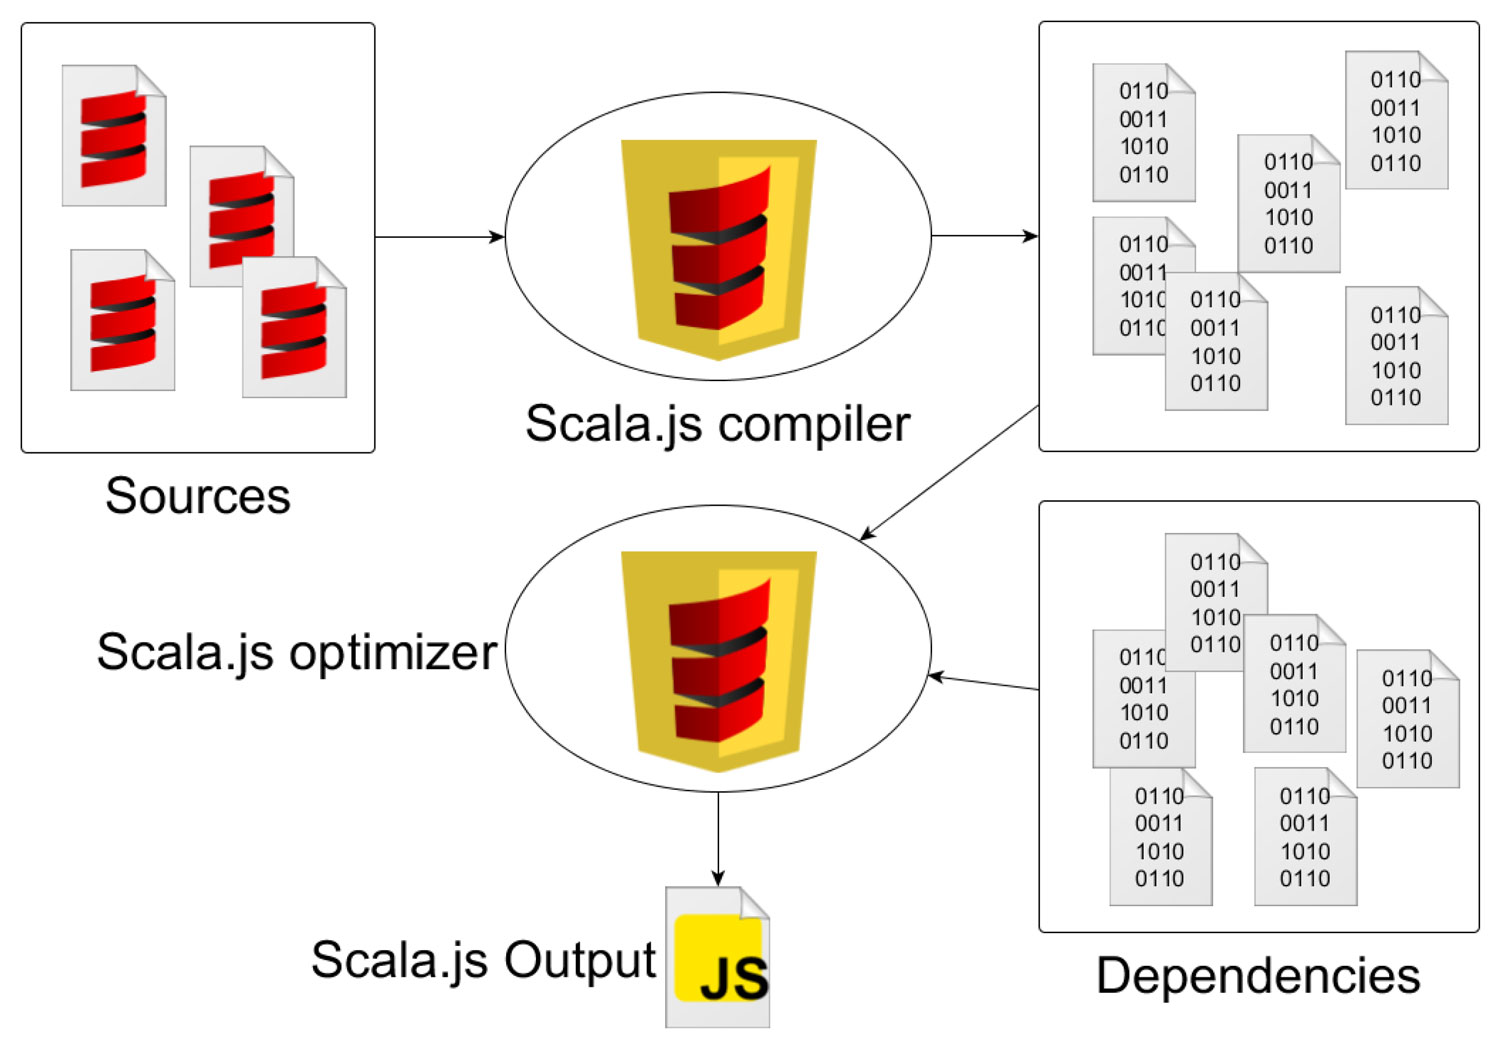
\includegraphics[width=0.75\textwidth]{Doeraene2014-Scalajs-p17}
    \caption[Der Scala.js-Kompilationsprozess]{Der Scala.js-Kompilationsprozess. \cite[Folie 17]{doeraene2014.WHB}}
    \label{fig:sjs-compilation}
\end{figure}

In der Optimierungsstufe (\code{FastOptJS}) wird unter anderem unerreichbarer Code entfernt (\emph{Dead code elimination}) und es werden Methoden- und insbesondere anonyme Funktionsaufrufe ge-inlined (\emph{Closure elimination}), das heißt die Aufrufe werden durch ihre Implementierungen ersetzt. Hierdurch wird die Größe der Kompilate verringert und die Performance verbessert. Das Ergebnis dieser Phase ist eine einzige JavaScript-Datei. Für die Entwicklungsphase endet der Prozess hier.

Zur weiteren Verringerung der Dateigröße gibt es nun noch eine Optimierungsphase (\code{FullOptJS}), bei welcher der Google Closure Compiler\footnote{\url{https://developers.google.com/closure/compiler/}} diese "`schnell-optimierte"' JavaScript-Datei durch weitere Dead code elimination, Entfernung von Whitespace sowie die aggressive Verkürzung von Variablennamen zusätzlich stark verkleinert. Dieser Optimierungsschritt ist allerdings nicht besonders schnell. Er ist deshalb für die Produktionsphase vorgesehen. \cite{scalajs.DCO}\cite[\#HowCompilationWorks]{haoyi.HOS}

Der Scala.js-Compiler unterstützt separate und inkrementelle Kompilierung, das heißt nur die einzelnen geänderten Kompilationseinheiten beziehungsweise sogar nur einzelne geänderte Programmteile innerhalb einer Datei werden neu übersetzt. Das beschleunigt inkrementelle Builds erheblich, was insbesondere dem gewohnten Workflow von Frontend-Entwicklern entsprechen dürfte.


\section{Stabilität}

Scala.js garantiert ab Version 0.6.0 Rückwärtskompatibilität, und zwar sowohl bezüglich der Semantik als auch für die Standardbibliothek\footnote{Dokumentation: \url{http://www.scala-js.org/api/scalajs-library/0.6.5/\#scala.scalajs.js.package}}, (die sowohl Quellcode- als auch binärkompatibel sein wird) und mit sbt erzeugte Builds (Quellcode-kompatibel). Einzig das Format für den Scala.js-spezifischen Zwischencode (.sjsir) könnte bis zur Version 1.0.0 noch einmal geändert werden. \cite{doeraene2015.SNL}

Die Scala Test-Suite läuft für knapp 2000 Tests, die das erwartungsgemäße Kompilieren beziehungsweise Nicht-Kompilieren prüfen, zu 99\% erfolgreich durch. Von über 1000 Tests, die die korrekte Ausführung überprüfen, sind 51 \% erfolgreich \cite[Folie~36, Min.~35]{doeraene2014.WHB}. Bei den wenigsten der Fehlschläge handelt es sich laut Doeraene allerdings tatsächlich um Bugs. Der Grund hierfür liegt darin, dass Scala.js bestimmte Spracheigenschaften wie Laufzeit-Reflections und die Java Collections nicht unterstützt \cite[S.~7]{doeraene2013.TDI}. Zusätzlich gibt es eine eigene Test-Suite mit über 400 Tests \cite[Folie 36, Min. 35]{doeraene2014.WHB}.


\section{Dokumentation}

Scala.js ist auf der offiziellen Website\footnote{\url{http://www.scala-js.org/}} dokumentiert. Hier findet sich die \ac{API}-Dokumentation, eine Referenzhandbuch sowie eine Übersicht über die mit Scala.js benutzbaren Librarys. Auch historische \ac{API}-Dokumentationen und  Release-Ankündigungen sind hier einsehbar.

Zum Einstieg gibt es ein Tutorial und beispielhafte Projektstrukturen (\emph{Skeletons}, die als Grundlage für eigene Projekte dienen können. Auch kann mit dem interaktiven Online-Scratchpad Scala.jsFiddle\footnote{\url{http://www.scala-js-fiddle.com/}} Scala.js direkt im Browser ausprobiert werden. Einige interessante Vortragsvideos der Scala.js-Entwickler sind hier verlinkt, es gibt ein FAQ, eine Mailingliste und einen eigenen Scala.js-Chatroom.

Es gibt bereits ein E-Book\footnote{\url{http://lihaoyi.github.io/hands-on-scala-js/}}, das mit vielen praktischen Beispielen einen guten Überblick über die Möglichkeiten von Scala.js liefert und auch grundlegende konzeptionelle Hintergründe erläutert.


\section{Ökosystem: Tools und Librarys}\label{sec:sjs-libs}

Obwohl das Projekt Scala.js noch ziemlich jung ist, existiert schon eine beachtliche Auswahl an Tools und Librarys. 


\subsection{sbt-Integration}\label{subsec:sjs-sbt}

Mit dem Scala.js-sbt-Plugin\footnote{\url{http://www.scala-js.org/doc/sbt-plugin.html}} ist es möglich, Scala.js-Anwendungen zu kompilieren, zu testen und auszuführen.
Prinzipiell kann auch auf sbt verzichtet und direkt mit einem Command Line Interface\footnote{\url{http://www.scala-js.org/downloads.html}} gearbeitet werden. Es wird jedoch empfohlen, sbt zu benutzen.

\TODOi{VGL: ...}
%-->  \url{http://www.scala-js.org/doc/tutorial.html}

\MyMiniSec{Projekt}

Die Ordnerstruktur für ein einfaches Scala.js-Projekt ist in Listing \ref{code:sjs-project-struct} dargestellt. Diese Ordnerstruktur muss per Hand angelegt werden. IntelliJ-Benutzer können sich auch ein sbt-Projekt generieren lassen, und dieses entsprechend anpassen. Alternativ bietet es sich an, eines der Skeletons zu verwenden, die auf der Scala.js-Website verlinkt sind. Eine andere Möglichkeit wäre es, sich ein kleines Skript zur Projekt-Generierung zu schreiben\footnote{Beispiele: siehe beigelegter Datenträger.}.

\begin{lstlisting}[caption={Struktur eines einfachen Scala.js Projekts.}, label={code:sjs-project-struct}]
myproject
 +- project
 |   +-- build.properties
 |   +-- plugins.sbt
 |- src
 |   +-- main
 |   |    +-- resources
 |   |    +-- scala
 |   +-- test
 |        +-- scala
 +- build.sbt
\end{lstlisting}

Das Scala.js-sbt-Plugin muss durch Eintrag \code{plugins.sbt} hinzufügt werden (Listing \ref{code:sjs-sbt-plugins}).

\lstinputlisting[language=Scala, caption={Eine minimale \code{plugins.sbt}.}, label={code:sjs-sbt-plugins}]{listings/setup/minimal_plugins.sbt}

Um das Scala.js-Plugin zu aktivieren, muss in der \code{build.sbt} eine entsprechende Zeile hinzugefügt werden. Außerdem darf die angebene Scala-Versionsnummer nicht kleiner als 2.10.2. Außerdem sollten Name und Versionsnummer für das Projekt festgelegt werden (Listing \ref{code:sjs-sbt-build}).

\lstinputlisting[language=Scala, caption={Eine minimale \code{build.sbt}.}, label={code:sjs-sbt-build}]{listings/setup/minimal_build.sbt}

Durch die letzte Zeile in der \code{build.sbt} wird für den \code{FastOptJS}-Modus Node.js als JavaScript-Laufzeit aktiviert. Hiermit laufen Aufrufe von der Kommandozeile sowie Tests schneller als mit dem langsameren Rhino. Allerdings muss dazu auch Node.js installiert sein.

\lstinputlisting[language=Scala, caption={Eine minimale \code{build.properties}.}, label={code:sjs-sbt-build-properties}]{listings/setup/minimal_build.properties}

In der \code{build.properties}-Datei muss die sbt-Version festlegen auf mindestens 0.13.7 eingestellt werden (Listing\ref{code:sjs-sbt-build-properties}).


\MyMiniSec{Dependencys}

Abhängigkeiten von Librarys werden in der \code{build.sbr} hinzugefügt, und zwar entweder so:

\begin{lstlisting}[style=snippet]
libraryDependencies += "org.scala-js" %%% "scalajs-dom" % "0.8.0"
\end{lstlisting}

oder, für mehrere Librarys, als \code{Seq}:

\begin{lstlisting}[style=snippet]
libraryDependencies ++= Seq(
  "org.scala-js" %%% "scalajs-dom" % "0.8.0",
  "be.doeraene" %%% "scalajs-jquery" % "0.8.0",
  "com.lihaoyi" %%% "scalatags" % "0.5.2",
  "com.lihaoyi" %%% "utest" % "0.3.1" % "test"
)
\end{lstlisting}

Für cross-publizierte Librarys muss der Operator \code{\%\%\%} (statt \code{\%\%}) verwendet werden. Für Librarys lässt sich auch ein Scope festlegen. Zum Beispiel wird durch nachgestelltes \code{\% "test"} für die betreffende Library Test-Scope definiert, das heißt die Library ist nur in diesem Modus verfügbar.

Wenn eine Scala.js-Fassade für eine JavaScript-Bibliothek als Dependency definiert ist, so wird die entsprechende JavaScript-Bibliothek automatisch geholt.

Der offiziellen Dokumentation\footnote{ \url{http://www.scala-js.org/doc/sbt/depending.html}} zufolge, sollte die Zeile:

\begin{lstlisting}[style=snippet]
skip in packageJSDependencies := false
\end{lstlisting}

in die \code{build.sbt} aufgenommen werden. Dadurch werden beim Build alle JavaScript-Dependencys in einer Datei (\code{-jsdeps.js}) gesammelt. Auf diese Weise muss nur \emph{eine} Datei für alle JavaScript-Dependencys in das \ac{HTML}-Dokument eingebunden werden. -- Den Erfahrungen im Rahmen dieser Arbeit nach, funktioniert dies sogar ganz ohne die zusätzliche Zeile in der Build-Definition.

Auch beliebige JavaScript-Bibliotheken können mittels WebJars\footnote{\url{http://www.webjars.org/}} geholt werden. So können auch minifizierte Alternativen der JavaScript-Librarys festgelegt werden. Soll dies beispielsweise für jQuery geschehen, so wird die folgende Zeile benötigt:

\begin{lstlisting}[style=snippet]
jsDependencies += "org.webjars" % "jquery" % "2.1.4" / "jquery.js" minified "jquery.min.js"
\end{lstlisting}

Eine Scala.js-Fassaden (wie \code{scalajs-jquery}), kann nun im \code{FullOptJS}-Modus auf die minifizierte Version von jQuery zurückgreifen. Diese wird passend in die Ausgabedatei \mbox{\code{-jsdeps.min.js}} integriert. Ohne diese explizite Angabe wird immer die nicht-minifizierte Version verwendet.


\MyMiniSec{sbt-Kommandos}

Mit sbt können folgende Kommandos aufgerufen werden:

\begin{itemize}
\item \code{run} kompiliert Scala.js-Anwendung und führt sie aus in einer JavaScript-Laufzeit aus. Dazu wird eine \code{main}-Methode benötigt.
\item \code{fastOptJS} wird zur Entwicklung benutzt. Für die erzeugten JavaScript-Dateien wird nur die erste Optimierungsstufe verwendet.
\item \code{fullOptJS} ist für die Produktion. Die erzeugten JavaScript-Dateien werden maximal auf kleine Dateigrößen hin optimiert.
\item \code{test} kompiliert den Code für Scala.js-Tests und führt sie aus. Außerdem werden im Verzeichnis \code{target/test-reports/} Test-Reports im \ac{XML}-Format erzeugt.
\item \code{compile} kompiliert zu Scala.js-Bytecode.
\item \code{package} packt Scala.js-Anwendung als .jar-Datei
\end{itemize}

Die JavaScript-Laufzeit ist, je nach Einstellung: Rhino, Node.js oder PhantomJS.

Durch eine vorangestellte \code{\~} ist das Arbeiten im kontinuierlichen Modus möglich
Jede gespeicherte Code-Änderung löst automatisch einen Neuaufruf des gewählten Tasks aus. Zum Beispiel wird mit \code{\~fastOptJS} automatisch im Produktionsmodus neu übersetzt. \cite[\#TheCommandLine]{haoyi.HOS} ist hier wieder eine wertvolle und (als Mitarbeiter des Projekts) auch autorisierte Quelle -> es gibt weiter unten ein Kapitel "`The Command Line"' zum Thema.

Die zur Auslieferung benötigten JavaScript-Dateien werden im Verzeichnis \code{target/scala-2.11/} erzeugt; \ac{HTML}- und \ac{CSS}-Dateien befinden sich eine Ebene tiefer in \code{target/scala-2.11/classes/}.




\subsection{IDE-Support}\label{subsec:sjs-ide}
(http://www.scala-lang.org/news/2015/02/05/scala-js-no-longer-experimental.html)

Scala.js kann gut durch \ac{IDE}s unterstützt werden. Hierdurch ist ein komfortableres Editieren durch Syntax-Hervorhebungen, intelligente automatische Code-Vervollständigungen, das Springen zur Definition, die Einblendung von Quellcode-Dokumentation und eine Unterstützung beim Refactoring möglich. \cite{doeraene2015.SNL} Infrage kommen folgende \ac{IDE}s:

\begin{description}
	\item[IntelliJ IDEA] liefert am meisten Komfort, unterstützt sbt schon am besten und ist deshalb klar die erste Wahl. Scala wird bei der aktuellen Version von Hause aus unterstützt, ältere Versionen lassen sich mit einem Plugin nachrüsten. sbt-Dateien werden erkannt und auch hier wird automatische Code-Vervollständigung unterstützt. Änderungen an sbt-Konfigurationsdateien werden von IntelliJ erkannt; das Programm schlägt dann einen "`Refresh"' vor. Zusätzlich kann direkt aus IntelliJ heraus mit dem Terminal gearbeitet werden\footnote{\url{https://www.jetbrains.com/idea/help/working-with-embedded-local-terminal.html}}. Die Ultimate Edition unterstützt außerdem auch JavaScript, \ac{HTML}, \ac{CSS}
	\item[Scala IDE / Eclipse] funktioniert recht gut. Allerdings fehlt sbt-Unterstützung.
	\item[Netbeans] kommt ebenfalls in Betracht, wurde allerdings nicht erprobt. Hierfür existiert ein Scala-Plugin.
\end{description}



\subsection{Scala.js workbench}

Die Scala.js workbench\footnote{\url{https://github.com/lihaoyi/workbench}} ist ein sbt-Plugin zur automatischen Aktualisierung des Browsers 
bei gespeicherten Änderungen am Code. Dies soll die kontinuierliche Entwicklung mit Scala.js erleichtern. Auch Ausgaben des Compilers werden in die Browser-Konsole übertagen.


\subsection{Librarys}

Hier sollen nur die Librarys kurz angesprochen werden, die im Rahmen dieser Arbeit zur Anwendung kamen. Einige davon sind JavaScript-spezifisch (zum Beispiel Scala-js-dom), aber die meisten laufen auf beiden Plattformen, JavaScript und \ac{JVM}. Viele Librarys befinden sind noch in einem frühen Entwicklungsstadium.

\begin{description}
	\item[Scala-js-dom]\footnote{\url{http://scala-js.github.io/scala-js-dom/}} bietet statische Typen für die komplette \ac{DOM}-\ac{API}. Damit sind unter anderem DOM-Manipulationen, die Verwendung des Canvas, von XMLHttpRequests, Drag and Drop, Websockets und localStorage möglich. Zusätzlich sind Komfort-Erweiterungen für Ajax-Requests und zum erleichterten Arbeiten mit Tastatur-Codes und Farben enthalten.
	
	\item[scala-js-jquery]\footnote{\url{https://github.com/scala-js/scala-js-jquery}} enthält statische Typen für die populäre jQuery-Library. Es existiert auch eine Alternative (\code{jquery-facade}), die aber nicht ausprobiert wurde.
	
	\item[ScalaTags]\footnote{\url{http://lihaoyi.github.io/scalatags/}} liefert eine \ac{DSL} zum komfortablen \ac{HTML}-Templating. Durch die Verwendung können unter anderem nicht-valide \ac{HTML}-Tags vermieden werden und die \ac{IDE}-Unterstützung für das Schreiben von \ac{HTML}-Elementen ist verbessert. Auch \ac{CSS} kann generiert werden; hierbei ist es sogar möglich, Stylesheets voneinander erben zu lassen. ScalaTags funktioniert für JavaScipt und auf der \ac{JVM}.

	\item[uTest]\footnote{\url{https://github.com/lihaoyi/utest}} (\emph{micro-test}) ist eine minimale cross-kompilierende Test-Library.
	
	\item[Scala-Async]\footnote{\url{https://github.com/scala/async}} ist eine Scala-Library zur einfacheren Handhabung von Asynchronität mit Futures. Sie funktioniert auch problemlos mit Scala.js.
	
	\item[Autowire]\footnote{\url{https://github.com/lihaoyi/autowire}} ist eine cross-kompilierende Library für statisch typisierte Netzwerkaufrufe. Hierfür muss zusätzlich eine Serialisierungs-Library festgelegt werden. Diese ist ebenso frei wählbar wie 
	
	\item[uPickle (?)]\footnote{\url{http://lihaoyi.github.io/upickle-pprint/upickle/}} ist eine cross-kompilierende Serialisierung-Library.
\end{description}



% % % % % % % % % % % % % % % % % % % % % % % % % % % % % % % %
\chapter{Methodik}\label{chap:methods}

An dieser Stelle soll die Vorgehensweise der Untersuchung erläutert werden. Zunächst müssen einige Kriterien aufgestellt werden, die bei der Einschätzung des Nutzens, den Scala.js bietet, helfen sollen. Dann soll das weitere Vorgehen erklärt werden. Schließlich wird kurz festgehalten, welche spezifischen Werkzeuge bei der Untersuchung konkret zum Einsatz kamen.

\section{Kriterien der Untersuchung}

Bei der Einschätzung des Gebrauchswerts von Scala.js sind zwei Blickwinkel zu berücksichtigen: einerseits der des Entwicklers, der Scala.js verwendet, andererseits der des Anwenders, für den eine Software mit Scala.js entwickelt wird.

\MyMiniSec{Entwicklersicht}

Aus Entwicklersicht steht die Frage im Vordergrund, wie Scala.js produktiv eingesetzt werden kann. Hierfür ist es zunächst wichtig die Handhabung zu verstehen. Dabei gilt es herauszufinden, auf welche Feinheiten zu achten ist, aber auch ob an bestehendes Wissen angeknüpft werden kann, kurz: wie hoch der Lernaufwand ist.

Für eine hohe Produktivität bei der Entwicklung ist der Komfort in der Handhabung von nicht zu unterschätzender Bedeutung. Dazu zählen die Unterstützung durch Programmierwerkzeuge und die Automatisierbarkeit von häufig wiederholten Entwicklungsschritten (zum Beispiel durch Buildtools). Hierbei ist die Schnelligkeit der Compiler-Läufe und Tests ein wichtiger Faktor in der alltäglichen Entwicklungsarbeit. Besonders Frontend-Entwickler sind hier schnelle Builds und ein inkrementelles Arbeiten gewohnt. Beim komplexen Prozess der Softwareentwicklung ist es wichtig, die Entwickler zielgerichtet bei ihrer Arbeit zu unterstützen. Hierfür ist eine gute Dokumentation relevant. Ebenso sollte der Aufwand für die effektive Konfiguration eines Projekts angemessen sein.

Entscheidend für die Produktivität bei der Entwicklung wie auch für die Qualität der Software ist die Code-Qualität. Robert C. Martin bezeichnet guten Code als eine der "`robustesten, am besten unterstützten und meistdiskutierten Prämissen unserer Zunft"' \cite[S. 27]{martin2009.CCH}. Schlechter Code lässt sich nur schwer ändern\footnote{In einer Negativ-Definition charakterisiert Martin schlechten Code drastisch als schwer zu durchschauendes "`Chaos"'.} und führt zu mehr schlechtem Code und einer asymptotisch abnehmenden Produktivität. Als häufigen Grund, für schlechten Code nennt Martin das Arbeiten unter Zeitdruck. \cite[S. 27 f.]{martin2009.CCH}

Dave Thomas macht Code-Qualität an folgenden Kriterien fest: "`Sauberer Code kann von anderen Entwicklern gelesen und verbessert werde. Er verfügt über Unit- und Acceptance-Tests. Er enthält bedeutungsvolle Namen. Er stellt zur Lösung einer Aufgabe nicht mehrere, sonder eine Lösung zur Verfügung. Er enthält minimale Abhängigkeiten, die ausdrücklich definiert sind, und stellt ein klares und minimales API zur Verfügung."' \cite[zit. nach: ][S. 35]{martin2009.CCH} Andere bekannte Programmierer beschreiben sauberen Code als "`möglichst elegant und effizient"' (Bjarne Stroustrup), "`einfach und direkt [...] wie wohlgeformte Prosa"' (Grady Brooch) und erkennen ihn an der "`Reduzierung der Duplizierung, Steigerung der Ausdrucksraft und frühe[n] Formulierung von Abstraktionen"' (Ron Jeffries) oder schlicht daran, dass er \emph{erwartungsgemäß} funktioniert (Ward Cunningham) \cite[alle zit. nach: ][S. 32 ff.]{martin2009.CCH}.

Das Entwickeln von Software besteht zu einem überraschend hohen Anteil im Lesen von schon bestehendem Code (laut Martin beträgt das Verhältnis über 10 : 1 \cite[S.~42]{martin2009.CCH}). Dadurch ist klar, welche besonders wichtige Rolle gerade die Lesbarkeit von Code spielt. Daneben sollen eine gute Wartbarkeit und Änderbarkeit, die Wiederverwendbarkeit von Code-Teilen, die Redundanzfreiheit, minimale Abhängigkeiten, die Erreichung von Testbarkeit und die Effizienz als Zielkriterien für eine hohe Code-Qualität festgehalten werden.

\MyMiniSec{Anwendersicht}

Andererseits sind auch verschiedene Kriterien zu berücksichtigen, welche die Sicht des Anwenders betreffen. Hier ist die Frage, ob Scala.js der Umsetzung von gängigen Anwendungsfällen Grenzen setzt. Neben der Machbarkeit ist es eine wichtige Grundbedingung für die Zufriedenheit der Anwender, dass sich Webseiten schnell anfühlen. Daraus resultieren verschiedene Anforderungen an die Leistungsfähigkeit von Weboberflächen. Erstens sollten Webseiten schnell laden. Hierzu muss die Datenmenge beim Laden einer Seite gering gehalten werden. Dafür sollten auch die von Scala.js erzeugten Dateien möglichst klein sein. Auch die Interaktionen, die die Webseite bietet, sollten schnell sein. Dazu müssen Reaktionen, zum Beispiel auf einen Knopfdruck oder auf das Absenden eines Formulars hin, asynchron behandelt werden. Die Oberfläche soll weiter bedienbar bleiben und nicht blockieren, wenn Daten von einem Server nachgeladen werden. Schließlich müssen für Operationen wie Berechnungen oder die Auswertung von Collections schnelle Ausführungszeiten sichergestellt sein.


\section{Vorgehensweise}

Viele der herangezogenen Qualitätskriterien sind nicht leicht quantifizierbar. Um trotzdem eine qualifizierte Beurteilung vornehmen zu können, sollen häufig auftretende Anforderungen im Bereich clientseitiger Web-Entwicklung in kleineren Fallbeispielen konkret prototypisch umgesetzt werden. Die dabei gewonnenen Erfahrungen sollen anhand der aufgestellten Kriterien diskutiert werden, um anhand dessen eine Einschätzung über die Nützlichkeit von Scala.js für das Anwendungsfeld zu treffen.


\section{Verwendete Hard- und Software}

Es wurde Windows 8.1 Pro auf einem System mit 64-Bit Intel Core i7-3517U Prozessor und 1,9 GHz Takt, 4 GB RAM und einem SSD-Laufwerk verwendet. Bei der Enwicklung wurde vorrangig mit IntelliJ IDEA (Ultimate Edition) und dem Editor Sublime Text 2 gearbeitet. Als Terminal wurde die git-bash vewendet, die in der Windows-Distribution von git enthalten ist.


\section{Messverfahren}

Zur Zeitmessung der Compiler- und Test-Läufe wurde auf die Zeitangaben von sbt zurückgegriffen.

Für die ermittelten Dateigrößen wurden die für den entsprechend Modus (\code{FastOptJS}, \code{FullOptJS} oder \code{test}) erzeugte JavaScript-Datei, die Source-Maps-Datei, die Datei mit den JavaScript-Dependencys sowie die benötigten \ac{HTML}- und \ac{CSS}-Dateien betrachtet. Andere Artefakte, wie der erzeugte Bytecode (\code{.class}- und \code{.sjsir}) wurden hier ignoriert.

Zur Messung der Ausführungsgeschwindigkeit von JavaScript-Programmen kam JSLitmus\footnote{\url{http://www.broofa.com/Tools/JSLitmus/}} mit Google Chrome (46.0.2490.80) zum Einsatz.



% % % % % % % % % % % % % % % % % % % % % % % % % % % % % % % %
\chapter{Projekt-Setup, Installation}\label{chap:setup}

Die nachfolgende Anleitung bezieht sich auf die Installation auf einem Windows-8.1-Rechner. Auf anderen Plattform können einzelne Schritte im Detail abweichen.

Um die Installation erfolgreich durchführen zu können ist eine gute Internetverbindung erforderlich, da die einige Bibliotheken heruntergeladen müssen. Außerdem wird ein aktueller Browser benötigt. Für volle Source-Maps-Unterstützung in der Browser-Konsole empfiehlt sich hier Google Chrome\footnote{\url{https://www.google.de/chrome/browser/desktop/}}.

\section{Benötigte Software}

Die folgende Software wird benötigt:

\begin{itemize}
	\item Java Development Kit (JDK) 8\footnote{Gegebenenfalls genügt auch ein JRE.}  --  \url{www.oracle.com/technetwork/java/javase/}
	\item Scala  --  \url{http://www.scala-lang.org/}
	\item sbt  --  \url{http://www.scala-sbt.org/}
	\item git  --  \url{https://git-scm.com/} \TODOi{<<<<< benötigt??? <<<<<}
	\item Node.js  --  \url{https://nodejs.org/en/}
	\item PhantomJS  --  \url{http://phantomjs.org/}
\end{itemize}

Alle benötigten Programme sind auf dem beigefügten Datenträger enthalten. Sie lassen sich alternativ auch unter der angegebenen Adresse beim Hersteller herunterladen. Dort finden sich auch Installationsanleitungen. Für Windows existieren ausführbare Installationsprogramme, die selbsterklärend sind. PhantomJS muss nicht installiert werden; hier genügt es, den Inhalt der .zip-Datei in das gewünschte Programmverzeichnis zu entpacken.

Unter Windows ist es für alle Programme \TODOi{mit Ausnahme von git} nötig, dem System durch das Setzen einer Umgebungsvariablen den Installationspfad bekannt zu machen.


\begin{enumerate}
\item "`System"'-Dialog öffnen (\code{Windows-Taste + x})
\item "`Erweiterte Systemeigenschaften"' mit Administrator-Rechten öffnen
\item Knopf "`Umgebungsvariablen"' betätigen
\item Variable "`Path"' auswählen und auf "`Bearbeiten..."' klicken
\item Pfad zur ausführbaren Datei des Programms (\code{bin/} im jeweiligen Programmverzeichnis) mit vorangestelltem Semikolon an bestehenden Eintrag anhängen, zum Beispiel für Java: \code{;C:\\Program Files\\Java\\jdk1.8.0\_51\\bin}
\end{enumerate}

Scala.js muss nicht installiert werden sondern wird per Build-Definition als sbt-Plugin gestartet.


\section{IDE-Integration}

Für die bequemere Navigation im Projekt bietet sich der Einsatz einer \ac{IDE} an (siehe Abschnitt: \ref{subsec:sjs-ide}).


\MyMiniSec{In IntelliJ importieren\footnote{Siehe auch: \url{https://www.jetbrains.com/idea/help/getting-started-with-scala-js.html}}}

\begin{enumerate}
\item File  >  New  >  "`Project from Existing Sources..."'
\item "`Select File ... to Import"'  >  Projektordner (mit \code{build.sbt}) auswählen  >  Ok
\item "`Import project from external model"' auswählen und auswählen  >  Next
\item "`Download sources and docs"' auswählen  >  Finish
\end{enumerate}

Nach Änderungen an sbt-Konfigurationsdateien ist ein "`Refresh"' in IntelliJ nötig.



\MyMiniSec{In Scala IDE importieren}

Für die Eclipse-basierte Scala IDE muss zuerst ein Eclipse-Projekt erzeugt werden. Hierzu ist das sbt-Plugin sbteclipse\footnote{\url{https://github.com/typesafehub/sbteclipse}} nötig. Dazu in \code{project/plugins.sbt} hinzufügen:

\begin{lstlisting}[language=Scala, style=snippet]
addSbtPlugin("com.typesafe.sbteclipse" % "sbteclipse-plugin" % "4.0.0")
\end{lstlisting}

Wenn sbteclipse versuchen soll, die Quellen der Library-Dependencys herunterzuladen, muss noch ein Eintrag in der \code{build.sbt} gemacht werden:

\begin{lstlisting}[language=Scala, style=snippet]
EclipseKeys.withSource := true
\end{lstlisting}

Im Anschluss diese Schritte ausführen:

\begin{enumerate}
\item \code{sbt eclipse} im Terminal ausführen. Dadurch werden
\code{.project} und \code{.classpath} erzeugt.
\item In der Scala IDE > File > Import > "`Existing Projects into Workspace"'
\item Projektordner auswählen > Finish
\end{enumerate}

Eclipse erzeugt standardmäßig ein Verzeichnis \code{bin/} im Projektwurzelverzeichnis, als Zielordner des Compilers.

Nach Änderungen an sbt-Konfigurationsdateien muss erneut \code{sbt eclipse} ausgeführt und das Projekt in Eclipse im Package Explorer aktualisiert werden.



\section{Installation von Source-map-support}

Um Source Maps verwenden zu können, sollte \emph{source-map-support}\footnote{\url{https://www.npmjs.com/package/source-map-support}} im Projekt installiert werden mit:

\begin{lstlisting}[style=snippet]
npm install source-map-support
\end{lstlisting}

Die Dateien des Plugins werden im Projektverzeichnis im Ordner \mbox{\code{node\_modules/}} abgelegt. Es ist auch möglich, das Projekt als Node.js-Projekt zu initialisieren:

\begin{lstlisting}[style=snippet]
npm -y init
npm install source-map-support --save-dev
\end{lstlisting}

Das hat den Vorteil, dass die benötigten Dependencys in einer Konfigurationsdatei verzeichnet werden. Künftig kann der \code{node\_modules/}-Ordner bedenkenlos gelöscht werden. Ein einfacher Aufruf von \code{npm install} genügt um alle benötigten Node.js-Pakete zu laden.


\section{Installation und Start von Anwendungen und Tests}

\TODOi{git??? -> Sourcen von Datenträger oder github(?) (-> git client), hierzu genügt der Aufruf git clone <repo> vom Terminal im gewünschten Verzeichnis}

Die Beispielanwendungen finden sich auf dem Datenträger im Order \code{source/}. Jedes Beispielprojekt enthält eine Readme-Datei mit allen nötigen Schritten.


% % % % % % % % % % % % % % % % % % % % % % % % % % % % % % % %
\chapter{Fallstudien}\label{chap:case-studies}

\TODOi{In den folgenden Fallstudien werden anhand kleiner Beispielimplementierungen die Themen Interaktion mit dem \ac{DOM}, das Arbeiten mit Events, die Verwendung des HTML5 Canvas, asynchrone Datenübertragung mit Ajax, die Möglichkeit der Erstellung cross-kompilierender Librarys und ein Beispiel für Client-Server Interaktion mit einem clientseitigen Routing vorgestellt. (CHECK!)} Ziel ist es dabei, bestimmte Aspekte der Nützlichkeit von Scala.js am jeweiligen Anwendungsfall zu zeigen und gegebenenfalls auf dabei aufgetretene Schwierigkeiten hinzuweisen.

Zuerst wird jeweils das Untersuchungsziel erläutert. Danach wird als zweites das Beispielprogramm kurz in seiner Funktionsweise beschrieben. Anschließend werden die Ergebnisse der Untersuchung besprochen und bewertet.

Das Eingangsbeispiel ist bewusst einfach gehalten, um in diesem Rahmen wichtige Eigenschaften von Scala.js zu diskutieren. Es stützt sich auf das offizielle Scala.js-Tutorial \cite{scalajs.SJT}. Für alle Implementierungen lieferten die Beispiele von Li Haoyi \cite{haoyi.HOS} wichtige Anregungen.

\TODO{Liste der Beispielprojekte, verlinkt auf GitHub}




% % % % % % % % % % % % % % % % % % % % % % % % % % % % % % % %
\section{Zwei Minimalbeispiele}

%TODO Hinweis: lose orientiert an  -->  http://www.scala-js.org/doc/tutorial.html

\TODO{Projekte: sjs-hello-scalajs, sjs-hello-scalajs2}

Ziel war es hier, anhand von zwei Minimalbeispielen verschiedene Grundbedingungen der Entwicklung mit Scala.js zu untersuchen. Dazu sollte als erstes ein klassischen Hallo-Welt-Programms zum Laufen gebracht werden. In diesem kleinen Rahmen sollte die grundlegende Handhabung und Konfiguration von Scala.js verstanden werden. Automatisierte Builds und einfache Tests sollten erprobt und auf ihre Performance hin untersucht werden. Auch die Größe der für die Auslieferung relevanten Kompilate sollte betrachtet werden.

Anhand eines weiteren minimalen Beispiels sollten einfache \ac{DOM}-Manipulationen, die Benutzerinteraktion mit Buttons und der Einsatz von jQuery ausprobiert und die Testbarkeit von Oberflächen-Elementen geklärt werden. Außerdem sollte die Source-Maps-Unterstützung zur Fehlersuche erprobt werden.


\MyMiniSec{Kurzbeschreibung des Hallo-Welt-Programms}

Das minimale Programm erzeugt die Ausgabe "`Hello world!"' in der Konsole des Browsers, wenn die entsprechende Webseite geöffnet wird. Der Aufruf \code{sbt run} erzeugt die gleiche Ausgabe in der sbt-\ac{REPL}. Der Scala-Code hierfür ist überschaubar, wie Listing \ref{code:hello.scala} zeigt.

\lstinputlisting[language=Scala, caption={Scala.js-Code für ein Hallo-Welt-Programm.}, label={code:hello.scala}]{listings/01hello-scalajs/HelloApp.scala}

\scala{HelloApp} erbt vom Trait \scala{JSApp}, der eine \scala{main}-Methode mit Rückgabetyp \scala{Unit} verlangt. Dadurch kann die \scala{HelloApp} mit ihrer \scala{main}-Methode nun in JavaScript unter ihrem voll qualifizierten Namen verwendet werden. Die Methode \scala{println} benutzt die Standardausgabe, das ist, je nach dem, von wo aus die Anwendung ausgeführt wird, die Browser-Konsole oder das sbt-\ac{REPL}.

Dieses Programm lässt sich bereits auf der sbt-Konsole ausführen (Listing \ref{code:run-hello}).

\begin{lstlisting}[caption={Lauf des Hallo-Welt-Programms in der sbt-REPL.}, label={code:run-hello}]
$ sbt
> run
[...]
[info] Updating {[...]/hello-scalajs/}hello-scalajs...
[info] Resolving [...] ...
[info] Done updating.
[info] Compiling 1 Scala source to [...]\hello-scalajs\target\scala-2.11\classes...
[info] Fast optimizing [...]\hello-scalajs\target\scala-2.11\hello-scalajs-fastopt.js
[info] Running hello.HelloApp
Hello world!
[success] [...]
\end{lstlisting}

Damit das kleine Programm im Browser ausgeführt werden kann, muß es in eine \ac{HTML}-Datei eingebunden werden, wie in Listing \ref{code:hello.html}.

\lstinputlisting[language=HTML5, caption={HTML-Code zur Einbindung der Scala.js-Datei in eine Website.}, label={code:hello.html}]{listings/01hello-scalajs/index-dev.html}


\MyMiniSec{Kurzbeschreibung des zweiten Programms}

Das erweiterte Minimalbeispiel erzeugt einen \code{<div>}-Container, der an den \code{<body>} des \ac{HTML}-Dokuments angehängt wird. An diesen Container werden verschiedene \ac{HTML}-Elemente angehängt, die vom Scala.js-Programm erzeugt werden: verschiedene \ac{HTML}-Elemente, die den Text "Hello world!" enthalten, sowie zwei Buttons. Die Buttons reagieren auf das Anklicken mit einer Text-Ausgabe sowohl auf die Browser-Konsole als auch in die Webseite. Einer der Buttons zählt, wie oft er angeklickt wurde und gibt die Anzahl bei der Ausgabe mit aus.


\MyMiniSec{Lernaufwand}

Für beide Minimalprogramme sowie für die Tests zum zweiten Programm diente das offizielle Scala.js-Tutorial\footnote{\url{http://www.scala-js.org/doc/tutorial.html}} als Grundlage. Diesem lässt sich sehr gut folgen. Grundkenntnisse in Scala, JavaScript, \ac{HTML} und im Umgang mit sbt sind allerdings hilfreich.


\MyMiniSec{Konfigurationsaufwand}

Es wird die für ein sbt-Projekt übliche Konfiguration (siehe Abschnitt \ref{sec:sbt}) bestehend aus \code{build.sbt} und \code{project/}-Verzeichnis mit \code{build.properties} benötigt. Zusätzlich muss in einer \code{plugins.sbt} im \code{project/}-Verzeichnis das Scala.js-Plugin hinzugefügt und dieses in der \code{build.sbt} aktiviert werden (siehe Abschnitt \ref{subsec:sjs-sbt}). Der Mehraufwand gegenüber einem reinen Scala-Projekt ist demnach gering. 


Die Einbindung von jQuery mit der Library \code{scala-js-jquery} ist grundsätzlich unkompliziert. Etwas schwieriger war es, zu verstehen, wie sich hier und generell minifizierte Versionen für die im \code{target/}-Ordner erzeugten JavaScript-Dependencys erzwingen lassen (siehe \ref{subsec:sjs-sbt}).


%TODO~~~~~


Für Tests wurde \code{uTest} verwendet und ensprechend den \code{libraryDependencies} hinzugefügt. Um das \ac{DOM} für Tests verwenden zu können, muss wie in \TODOi{Kapitel sbt-Integration ???} beschrieben, der Eintrag:

\begin{lstlisting}[style=snippet]
jsDependencies in Test += RuntimeDOM
\end{lstlisting}
in der Build-Definition ergänzt werden.

Um Source-Maps-Unterstützung im Browser zu bekommen, muss eine nicht allzu aufwendige Installation vorgenommen werden, wie in \TODOi{Abschnitt Source Maps ???} beschrieben. \TODOi{besser auslagern in eigenes Kapitel}

\MyMiniSec{Performance von Build und Tests}

Hier wurde die Geschwindigkeit der Build- und Test-Läufe sowie die Größe der Kompilate untersucht. \code{test} wurde immer in der FastOpt-Stage mit PhantomJS verwendet. Zwischen den Testläufen wurde nie \code{clean} aufgerufen. Für den ersten Testlauf existierte kein target-Ordner beziehungsweise dieser wurde zuvor gelöscht. Die Ergebnisse der Untersuchung sind in den Tabellen \ref{table:compiler-performance1} und \ref{table:compiler-performance2} dargestellt. Die verwendeten Abkürzungen sind in der Legende \ref{table:compiler-performance-legend} aufgeschlüsselt.

\medskip

\begin{table}[!h]
\begin{tabular}{|l|r|r|r|r|r|r||r|r|r|r|}
\hline           & $t_1$ & $t_2$ & $t_3$ & $t_4$ & $t_c$         & $t_n$ & $s_0$          & $s_1$  & $s_m$ & $s_d$ \\ 
\hline fullOptJS & 10 s  &  4 s  &  3 s  &  3 s  &          2 s  & 0-1 s & \textbf{20 kB} &  77 kB & 57 kB &  0 kB \\ 
\hline fastOptJS &  7 s  &  3 s  &  3 s  &  2 s  &  \textbf{2 s} & 0-1 s &        101 kB  & 193 kB & 92 kB &  0 kB \\ 
\hline 
\end{tabular} 
\caption{Build-Performance für ein minimales Hallo-Welt-Programm.}
\label{table:compiler-performance1}
\end{table}

\begin{table}[!h]
\begin{tabular}{|l|r|r|r|r|r|r||r|r|r|r|}
\hline           & $t_1$ & $t_2$ & $t_3$ & $t_4$ & $t_c$         & $t_n$ & $s_0$          & $s_1$  & $s_m$  & $s_d$ \\ 
\hline fullOptJS & 15 s  &  7 s  &  5 s  &  5 s  &          4 s  & 0-1 s & \textbf{57 kB} & 230 kB & 173 kB &   0 kB \\ 
\hline fastOptJS & 11 s  &  5 s  &  4 s  &  4 s  &  \textbf{3 s} & 0-1 s &        277 kB  & 520 kB & 243 kB &   0 kB \\ 
\hline test      & 35 s  & 24 s  & 24 s  & 22 s  &         19 s  &  16 s &        1,6 MB  & 2,8 MB & 1,2 MB & 241 kB \\ 
\hline 
\end{tabular} 
\caption{Build-Performance für ein leicht erweitertes Hallo-Welt-Programm mit Tests.}
\label{table:compiler-performance2}
\end{table}

\begin{table}[!h]
\begin{tabular}{|l|l|}
\hline $t_1$ & Dauer des 1. Compilerlaufs (target-Ordner existiert noch nicht) \\ 
\hline $t_2$ & Dauer des 2. Compilerlauf nach einem \code{clean} \\ 
\hline $t_3$ & Dauer des 3. Compilerlauf nach einem \code{clean} \\ 
\hline $t_4$ & Dauer des 4. Compilerlauf nach einem \code{clean} \\ 
\hline $t_c$ & Dauer ab 2. Compilerlauf mit Code-Änderungen ohne \code{clean} \\ 
\hline $t_n$ & Dauer ab 2. Compilerlauf ohne Code-Änderungen ohne \code{clean} \\ 
\hline $s_0$ & Größe der erzeugten Dateien ohne Source Maps \\ 
\hline $s_1$ & Größe der erzeugten Dateien mit Source Maps \\ 
\hline $s_m$ & Größe der erzeugten Source-Maps-Datei \\ 
\hline $s_d$ & Größe der erzeugten Datei, die die JavaScript-Dependencys enthält \\ 
\hline 
\end{tabular} 
\caption{Legende zu \ref{table:compiler-performance1} und \ref{table:compiler-performance2}.}
\label{table:compiler-performance-legend}
\end{table}

Es wird deutlich, dass sich der Compiler ab dem zweiten Lauf "`stabilisiert"' und selbst nach einem \textbf{clean} deutlich schneller fertig ist als beim ersten Lauf. Der für den Entwicklungsalltag häufiste Fall dürfte wohl ein Build nach Code-Änderungen ohne \textbf{clean} sein. Dafür sind 3 Sekunden eine vertretbare Zeit. Bei einem weniger trivialen Beispiel mit mehr Code wachsen diese Zeiten, bleiben aber den Erfahrungen im Laufe dieser Arbeit nach in der Regel unter \TODOi{10 Sekunden (CHECK --> clientserver oder stringanalyzer)} und damit in einem vertretbaren Rahmen.

Es ist auch zu erkennen, dass Testläufe, selbst ohne Code-Änderungen nicht besonders schnell sind. In den insgesamt 7 Tests werden 25 Assertions verwendet.\footnote{Im Code stehen 13 Assertions, davon werden 3 jeweils in einer Schleife 5-mal aufgerufen.} Schnellere Testläufe wären hier in jedem Fall wünschenswert. Andererseits fallen etwas langsamere Tests nicht ganz so stark ins Gewicht, wenn man im kontinuierlichen Modus arbeitet (zu erreichen mit dem Kommando \code{\~test}).

Die Größe der Kompilate für das Hallo-Welt-Programm übertrifft reines \ac{HTML}/JavaScript (187 Bytes) um einen Faktor von etwa 100. Dieses Ergebnis muss erklärt werden. Einen großen Teil der von Scala.js generierten JavaScript-Datei macht die Scala-Standardbibliothek aus. Der Optimierer reduziert die Code-Menge sehr stark (siehe Abschnitt \ref{sec:compiler}). Die Größe von optimiertem Scala.js-generierten JavaScript-Dateien wird deshalb mit wachsender Code-Basis des eigenen Software-Projekts nicht etwa proportional, sondern langsamer anwachsen. Haoyi verweist in diesem Zusammenhang auf ein eigenes Projekt mit einem Umfang von ca. 2000 Zeilen Code, welches voll optimiert noch 288 kB groß ist. \TODOi{-> vgl. eigenes client-server-Bsp.} Das Problem wird weiter relativiert durch die Tatsache, dass die meisten Server ihre Daten gzip-komprimiert übertragen, was laut Haoyi die Datenlast auf etwa ein Zehntel verkleinert. \cite[\#BlobSize]{haoyi.HOS}

Seit Bestehen des Projekts wurden bei der Verringerung der erzeugten Dateigröße schon erhebliche Fortschritte erzielt. Generierte der Prototyp des Compilers für ein Hallo-Welt-Programm noch 16 MB, so reduzierte sich dies bald darauf mit der Einführung des Google Closure Compilers ins Projekt im August 2013 schon auf 900 kB \cite[Folie~5~f., Min.~6]{doeraene2014.WHB}. Der aktuelle Stand mit 20 kB (siehe Tabelle \ref{table:compiler-performance1}) ist somit relativ gut und lässt auf weitere Verbesserung in der Zukunft hoffen.


\MyMiniSec{Debugging-Qualitäten}

Eine einfache Art des Debuggings besteht im Schreiben in die Konsole. Es funktioniert mit Scala.js hervorragend, mit \scala{println} einfache Ausgaben auf die Browser-Konsole zu machen. Möchte man allerdings den Inhalt von Objekten inspizieren, so genügt das häufig nicht. Angenommen sei eine Klasse \scala{class A(foo: Int, bar: String)} von der eine Instanz \scala{foo(123, "baz")} existiert. Der Aufruf \scala{println(foo)} generiert für Klassen, deren \scala{toString}-Methode nicht überschrieben wurde die lapidare Ausgabe \js{[object Object]}. Stattdessen kann hier mit \scala{dom.console.log} direkt die Browser-Konsole adressiert werden, um das Objekt zu inspizieren (\js{Object Ausgabe: {foo: 123, bar: "baz"}}). Besonders tiefer verschachtelte Strukturen lassen sich so sehr komfortabel untersuchen.

Besonders der Einsatz von Source Maps\footnote{Eine generelle Erläuterung zu Source Maps findet sich hier: \url{http://www.html5rocks.com/en/tutorials/developertools/sourcemaps/}} aber erhöht den Komfort beim Debugging in der Konsole des Browsers\footnote{Erprobt wurde hierbei Chrome.} erheblich. Durch Anklicken der entsprechenden Zeile im Stacktrace in der Browser-Konsole kann hierbei zur richtigen Zeile in der Ursprungsdatei navigiert werden. Selbst beim nicht-minifizierten Entwicklungs-Code macht es einen erheblichen Unterschied aus, ob man zur originalen Scala-Code springen kann, oder ob man gezwungen ist, compilergeneriertes JavaScript zu verstehen. Ein Vergleich der Abbildungen \ref{fig:no-sourcemaps} und \ref{fig:sourcemaps} macht den Unterschied deutlich. Selbst im \code{FullOptJS}-Modus funktioniert die Auflösung der Referenzen zum Scala-Code.

\begin{figure}[!h]
	\centering
	\subfloat[][]{
		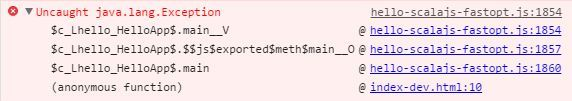
\includegraphics[width=0.66\textwidth]{sourcemaps1-dumb-stacktrace}
		\label{fig:sourcemaps1}
	}
	\subfloat[][]{
		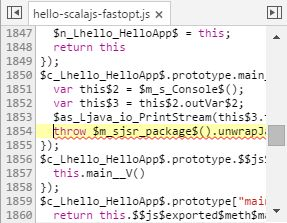
\includegraphics[width=0.33\textwidth]{sourcemaps2-cryptic-code}
		\label{fig:sourcemaps2}
	}
	\caption[Ohne Source Maps.]{Ohne Source Maps: Wenig aussagekräftiger Stacktrace \protect\subref{fig:sourcemaps1}, navigierbar zu schwer verständlichem, generierten JavaScript-Code \protect\subref{fig:sourcemaps2}.}
	\label{fig:no-sourcemaps}
\end{figure}

\begin{figure}[!h]
	\centering
	\subfloat[][]{
		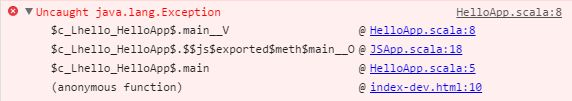
\includegraphics[width=0.66\textwidth]{sourcemaps3-smart-stacktrace}
		\label{fig:sourcemaps3}
	}
	\subfloat[][]{
		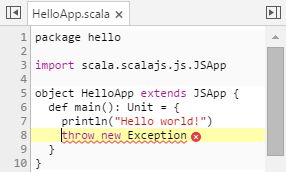
\includegraphics[width=0.33\textwidth]{sourcemaps4-legible-code}
		\label{fig:sourcemaps4}
	}
	\caption[Unterstützung durch Source Maps.]{Unterstützung durch Source Maps: Diagnosestärkerer Stacktrace \protect\subref{fig:sourcemaps3}, navigierbar zu verständlichem Scala-Code \protect\subref{fig:sourcemaps4}.}
	\label{fig:sourcemaps}
\end{figure}


\MyMiniSec{Testbarkeit}

Mit der Bibliothek uTest lassen sich Unit-Tests formulieren. Mit verschieden Macros (siehe Listing \ref{code:hallo-test}) kann etwa die Geschäftslogik und auch, wie beim zweiten Beispielprogramm geschehen, das korrekte Verhalten der Oberfläche getestet werden. Hier wurde geprüft, dass \ac{HTML}-Elemente wie erwartet existieren oder dass Buttons erwartungsgemäß reagieren. Allerdings ist es hierfür nötig, die betreffenden \ac{HTML}-Elemente mit eindeutigen IDs zu versehen, was einen zusätzlichen Overhead darstellt. Für eine leichtere Selektion von \ac{HTML}-Elementen in Tests erweist sich darüber hinaus der Einsatz von jQuery als nützlich. Was hier fehlt, ist die Möglichkeit, wie im JavaScript-Test-Framework Jasmine, mithilfe sogenannter \emph{Spies} prüfen zu können, ob und mit welchen Argumenten eine Methode aufgerufen wurde.\footnote{\url{http://jasmine.github.io/2.0/introduction.html\#section-Spies}} Für Scala.js existiert zwar ein Wrapper für Jasmine. In einer Ankündigung auf der offiziellen Scala.js-Webseite \cite{scalajs.ASJ} wird aber explizit von dessen Verwendung abgeraten.

\begin{lstlisting}[language=Scala, caption={Eine beispielhafte Test-Suite mit uTest.}, label={code:hallo-test}]
object MyTest extends TestSuite {
  override def tests = TestSuite{
    "foo" - {
      /* erwartet, das eine Bedingung true ist */
      assert(1 + 1 == 2)
      
      /* erwartet ein bestimmtes Pattern */
      assertMatch(List(1, 2, 3)){case 1 :: _ => }
      
      /* erwartet das Auftretetn der entsprechenden Exception */
      intercept[NoSuchElementException](Nil.head)
      
      /* erwartet einen Compiler-Fehler */
      compileError("val x: Int = 1.2")
    }
  }
}
\end{lstlisting}

Auch asynchrone Tests mit Futures sollen möglich sein, wurden aber nicht erforscht.

Grundsätzlich lässt sich mit uTest gut arbeiten, allerdings erhält man beim Fehlschlagen von Tests häufig einen sehr langen Stacktrace. Für einen größeren Komfort wäre hier für die Zukunft ein IDE-Plugin mit navigierbarem Stacktrace wünschenswert. Das Arbeiten im kontinuierlichen Testmodus (\code{\~test}) liefert unmittelbares Feedback auf alle vorgenommen Änderungen und ist damit ein sehr nützliches Werkzeug.


Die bekannten Test-Bibliotheken ScalaTest und Specs2 können nicht mit Scala.js verwendet werden, da sie zu stark von Java-Spezifika abhängen, um nach Scala.js portiert werden zu können. Allerdings gibt es noch eine Reihe anderer Test-Librarys, die für Scala.js einsetzbar ist. \cite[\#OtherTestingLibraries]{haoyi.HOS}






% % % % % % % % % % % % % % % % % % % % % % % % % % % % % % % %
\section{HTML-Templating}

%TODO -----> Kapitel raus, Wichtiges übernehmen in StringAnalyzer

\TODO{Projekte: sjs-hello-scalatags (+ extract: string-analyzer}

%\subsection{Ziel der Untersuchung}

\TODO{Ziel formulieren}

Typsicheres \ac{HTML}-Templating 

TODO: Einleitungssatz

%\subsection{Kriterien}

\begin{itemize}
	\item Machbarkeit
	\item Lesbarkeit
\end{itemize}

minisec{Kurzbeschreibung des Beispielprogramms}

Verschiedene valide \ac{HTML}-Tags werden mit Scala.js erzeugt.

minisec{Ergebnisse der Untersuchung und Bewertung}

Betrachtet wurden vier Möglichkeiten, in Scala.js \ac{HTML} zu generieren. Dazu sei in der \code{index.html} ein
\html{<div>} mit der ID "`container"' definiert. Die Referenz darauf wird im Scala.js-Programm bekannt gemacht durch:

\begin{lstlisting}[language=Scala, style=snippet]
val container: org.scalajs.dom.raw.Element = document.getElementById("container")
\end{lstlisting}

Mithilfe von Scala-js-dom können die \ac{DOM}-Methoden \scala{createElement()} zum erzeugen von \ac{HTML}-Elementen und \scala{appendChild()} zum einhängen von Elementen in den DOM-Tree verwendet werden.

\begin{lstlisting}[language=Scala, caption={HTML-Generierung mit Scala-js-dom und Nodes.}]
val foo = document.createElement("div")
foo.id = "hello-div"
foo.classList.add("first")
foo.setAttribute("style", "color: red;")
val par = document.createElement("p")
val txt = document.createTextNode("hello")
div.appendChild(par)
node.appendChild(elm)
\end{lstlisting}

Allerdings können so auch, ob absichtlich oder durch Tippfehler, nicht-valide \ac{HTML}-Elemente erzeugt werden, wie zum Beispiel diese:
\begin{lstlisting}[language=Scala, style=snippet]
document.createElement("xyz")     // --> <xyz>...</xyz>
document.createElement("\@\$#!")  // --> Laufzeitfehler
\end{lstlisting}

Eine weitere Möglichkeit, ist die direkte Manipulation der \code{innerHTML}-Property, der \ac{HTML}-Code als String zugewiesen werden kann.

\begin{lstlisting}[language=Scala, caption={HTML-Generierung mit Scala-js-dom und Strings.}]
node.innerHTML = s"""
 |<div id="hello-div" class="first" style="color: red;">
 |  <p>hello</p>
 |</div>
""".stripMargin
\end{lstlisting}

Bei dieser Variante sind aus Tippfehlern resultierende unvalide \ac{HTML}-Tags sogar noch wahrscheinlicher. Haoy warnt in diesem Zusammenhang auch vor der Gefahr von Cross-Site-Scripting \cite[\#HelloWorld:HTML]{haoyi.HOS}.

Mit ScalaTags nun ist es möglich, in Scala typsichere \ac{HTML}-Templates zu schreiben, aus denen sich valider \ac{HTML}-Code generieren lässt. Attribute wie etwa \code{id} und \code{class} können ebenso wie \ac{CSS}-Styles gesetzt werden.\footnote{ScalaTags bietet bei Bedarf sogar eine \ac{DSL}, um \ac{CSS}-Stylesheets zu generieren.}

Eine Möglichkeit ist es nun, aus diesen Templates \ac{HTML}-Strings zu rendern, was vor allem für serverseitiges \ac{HTML}-Templating interessant ist (hier existiert schließlich kein \ac{DOM}). In dieser Variante kann ScalaTags auch in reinen Scala-Projekten eingesetzt werden.

\begin{lstlisting}[language=Scala, caption={HTML-Generierung mit ScalaTags und Strings.}]
import scalatags.Text.all._
node.innerHTML =
  div(id:="hello-div", cls:="first", color:="red",
    p("hello")
  ).render
\end{lstlisting}

Für die Client-Seite existiert zusätzlich die bessere Möglichkeit, die Templates direkt in \scala{dom.Element}s umzuwandeln:

\begin{lstlisting}[language=Scala, caption={HTML-Generierung mit ScalaTags und Nodes.}]
import scalatags.JsDom.all._
node.appendChild(
  div(id:="hello-div", cls:="first", color:="red",
    id:="hello-div",
    p("hello")
  ).render
)
\end{lstlisting}

Damit ist es möglich typsicher, deklarativ und nahe an \ac{HTML}, gleichzeitig (schon durch das Wegfallen der schließenden Tags) sehr lesbaren Code zu schreiben. Hinzu kommt die Möglichkeit, Kontrollfluss-Anweisungen wie \scala{for} und \scala{if/else} einzustreuen (ein Beispiel hierfür: Listing \ref{code:setupCurrencySelect}).



% % % % % % % % % % % % % % % % % % % % % % % % % % % % % % % %
\section{Canvas, Timer und Events}

\TODO{Projekt: sjs-canvas-frenzy}

\TODO{>> Workbench ausgliedern!!!}

%\subsection{Ziel der Untersuchung}

Bei diesem Beispiel ging es um die Erprobung des HTML5-Canvas und der \ac{DOM}-\ac{API} mit Scala.js. Es sollten Timer-gesteuerte Aktionen mithilfe der Methoden des \code{WindowTimers}-Interface und das Arbeiten mit Event-Handlern für Maus- und Keyboard-Events ausprobiert werden. Hierbei sollte einerseits geklärt werden, ob und wie solche Standardtechniken der Oberfächenprogrammierung mit Scala.js machbar sind, andererseits sollte untersucht werden, ob die Entwicklung durch die Arbeit mit Scala.js sogar erleichtert wird, oder ob das Gegenteil der Fall ist.

Gleichzeitig wurde die Scala.js Workbench im produktiven Einsatz ausprobiert und dabei auf ihre Nützlichkeit hin geprüft.

%\subsection{Kriterien}

\begin{enumerate}
	\item Umsetzbarkeit aller Anforderungen
	\item Leichtigkeit der Implentierung
	\item Nützlichkeit
\end{enumerate}

\MyMiniSec{Kurzbeschreibung des Beispielprogramms}

Die Anwendung erzeugt automatisch einfache Bilder, indem sie zufällig Rechtecke oder Kreise von zeichnet. Auch Position, Abmessungen, Farbe und Transparenz der Elemente sind zufallsgeneriert. Bei den Abmessungen sorgt ein Mechanismus dafür, dass die Werte nicht zu abrupt variieren, sondern sich ein etwas ruhigerer Eindruck ergibt. Dazu werden die Zufallswerte jeweils durch lineare Interpolation mit dem letzten Wert geglättet. Das Ergebnis ist beispielhaft in den Abbildungen \ref{fig:frenzy1} und \ref{fig:frenzy2} zu sehen.

Mit der Maus kann bei gedrückt gehaltener linker Maustaste auf den Canvas-Bereich gezeichnet werden. Dabei wird ein zufälliger Farbverlauf erzeugt (siehe Abb. \ref{fig:frenzy3} und \ref{fig:frenzy4}).

\begin{figure}[!h]
	\centering
	\subfloat[][Kurz nach Start.]{
		
\includegraphics[width=0.46\textwidth]{canvas-frenzy/frenzy-snap01}
		\label{fig:frenzy1}
	}
	\quad
	\subfloat[][Nachdem etwas Zeit vergangen ist.]{
		
\includegraphics[width=0.46\textwidth]{canvas-frenzy/frenzy-snap02}
		\label{fig:frenzy2}
	}
	\qquad
	\subfloat[][Zeichnen mit Gradienten-Stift bei angehaltenem Auto-Zeichnen.]{
		
\includegraphics[width=0.46\textwidth]{canvas-frenzy/frenzy-snap03}
		\label{fig:frenzy3}
	}
	\quad
	\subfloat[][Auto-Zeichnen und Gradienten-Stift.]{
		
\includegraphics[width=0.46\textwidth]{canvas-frenzy/frenzy-snap04}
		\label{fig:frenzy4}
	}
	\caption{Screenshots der Canvas-Beispielanwendung.}
	\label{fig:frenzy}
\end{figure}

Die Anwendung lässt sich durch die Tastatur steuern. Das automatische Zeichnen kann durch Betätigen der Leertaste angehalten und wieder gestartet werden. Durch Betätigen der Escape-Taste wird die Zeichenfläche geleert. Die Geschwindigkeit, mit der neue Elemente gezeichnet werden, kann durch die Pfeil-Tasten gesteuert werden: "`nach oben"' beschleunigt das Neuzeichnen, "`nach unten"' verlangsamt es.

Die Größe der Zeichenfläche wird jeweils an die aktuelle Größe des Browserfensters neu angepasst. Allerdings wird dabei auch die Zeichenfläche geleert.

Eine Schwäche der aktuellen Implementierung ist es, dass die beim Zeichnen mit der Maus entstehende Linie bei langsamer Mausbewegung noch nicht sehr glatt erscheint. Das hängt damit zusammen, dass für jede registrierte Mausbewegung, die als MouseEvent verarbeitet werden kann, eine Teillinie gezeichnet wird. Diese ist jeweils die Verbindungslinie zwischen der Mausposition des vorigen mit der des aktuellen MouseEvent. Zwischen diesen Teillinie entsteht, wenn sie nicht in exakt dieselbe Richtung weisen, eine Lücke.

Ein anderer bekannter Fehler ist das ungewöhnliche Verhalten der Zeichenfläche beim Zoomen im Browser. \REDOi \TODOi{raffen und in einen Absatz}


%\subsection{Ergebnisse der Untersuchung und Bewertung}

Alle geplanten Anforderungen ließen sich umsetzen: der Zugriff auf die \ac{DOM}-\ac{API}, das Zeichnen auf den Canvas, timergesteuerte Ausführung und die Verwendung von Event-Handlern.

Um ein Canvas-Objekt zu erhalten, gibt es in JavaScript zwei Möglichkeiten: entweder man definiert im \ac{HTML}-Dokument ein Canvas-Element mit einer eindeutigen ID \html{<canvas id="myCanvas"></canvas>} und greift im JavaScript-Code darauf zu:

\begin{lstlisting}[language=JavaScript, style=snippet]
var canvas = document.getElementById("my-canvas")  // JavaScript
\end{lstlisting}

oder man erzeugt das Canvas-Element mit der \js{createElement}-Methode:

\begin{lstlisting}[language=JavaScript, style=snippet]
var canvas = document.createElement("canvas")      // JavaScript
\end{lstlisting}

Um diese Methoden der \ac{DOM}-\ac{API} in Scala.js zu verwenden, existiert die Bibliothek Scala-js-dom. Damit können die benötigten \ac{DOM}-\ac{API}-Methoden erwartungsgemäß verwendet werden:

\begin{lstlisting}[language=Scala, style=snippet]
val canvas = dom.document.getElementById("my-canvas").
  asInstanceOf[html.Canvas]
\end{lstlisting}

und in der Variante mit \scala{createElement}:

\begin{lstlisting}[language=Scala, style=snippet]
val canvas = dom.document.createElement("canvas").
  asInstanceOf[html.Canvas]
\end{lstlisting}

Zu beachten ist hier der Cast mit \scala{asInstanceOf[T]}. Die Methoden \scala{getElementById} und \scala{createElement}
geben nämlich ein Objekt vom Typ \scala{org.scalajs.dom.raw.Element} zurück. Der Cast ist also notwendig, um auf die Canvas-Methoden zuzugreifen. Er ist auch legitim, denn hier ist bekannt, dass es sich um ein Canvas-Objekt handeln muss.

Zum Zeichnen wird nun der 2D-Kontext benötigt. Auch hier ist aus den genannten Gründen ein Cast notwending. Danach kann der Kontext wie gewohnt verwendet werden.\footnote{Zum Zeichnen auf den Canvas siehe: \url{https://developer.mozilla.org/en-US/docs/Web/API/CanvasRenderingContext2D}}

\begin{lstlisting}[language=Scala, style=snippet]
val ctx = canvas.getContext("2d").
  asInstanceOf[dom.CanvasRenderingContext2D]
ctx.fillStyle = "silver"
ctx.fillRect(x, y, width, heigth)
\end{lstlisting}

Die Typ-Casts mögen etwas unschön sein, aber die zwei beschriebenen Fälle sind auch die einzigen, die in der Beispielanwendung benötig werden. Sébastien Doeraene zufolge ist die erste Art Cast zur Spezialisierung des \ac{HTML}-Elements, unvermeidbar, andernfalls müsste der \ac{DOM} selbst Teil des Typsystems sein. Der zweite Cast zum konkreten Rendering-Kontext wird wohl in einer künftigen Version von Scala.js nicht mehr nötig sein. Doeraene weist auch darauf hin, dass in sechs Scala.js-Beispielanwendungen mit insgesamt 1000 Zeilen Code exakt diese beiden Casts, und nur diese, benötigt werden. \cite[S. 8]{doeraene2013.TDI}

Um einen Timer zu starten, der ein Aktion regelmäßig ausführt, bietet die \ac{DOM}-\ac{API} die Methode \scala{setInterval}. Die folgende Anweisung erzeugt zum Beispiel einmal pro Sekunde eine Ausgabe auf die Konsole:

\begin{lstlisting}[language=JavaScript, style=snippet]
setInterval(function(){ console.log("hi"); }, 1000);  // JavaScript
\end{lstlisting}

In Scala.js lässt sich das nun recht ähnlich ausdrücken:

\begin{lstlisting}[language=Scala, style=snippet]
dom.setInterval(() => println("hi"), 1000)
\end{lstlisting}

Hier ist also nichts neu zu lernen, die JavaScript-\ac{DOM}-\ac{API} wird mithilfe der Fassade einfach verwendet. Zusätzlich profitiert man hier von der prägnanten Scala-Syntax, mit der sich Lambas knapper schreiben lassen.

Zur Veranschaulichung der Verwendung von Event-Handler sei hier folgendes Beispiel herausgegriffen:

\begin{lstlisting}[language=Scala, style=snippet]
dom.document.onkeyup = { (evt: dom.KeyboardEvent) => evt.keyCode match {
  case KeyCode.space =>  timer.toggle()
  case KeyCode.up =>     timer.decr()
  case KeyCode.down =>   timer.incr()
  case KeyCode.escape => clear()
  case _ => ()
}}
\end{lstlisting}

Hier wird der \scala{onkeyup}-Property zur Event-Behandlung eine anonyme Funktion (auch: Lambda) zugewiesen. Dank Scalas Pattern Matching kann sehr knapp und übersichtlich das gewünschte Verhalten formuliert werden. Scala-js-dom stellt neben Fassaden für die \ac{DOM}-\ac{API} im Paket \scala{org.scalajs.dom.ext} nützliche Helfer zur Verfügung, darunter eine Liste für die meisten Keyboard-Tasten-Codes, so dass hier nicht mit kryptischen Zahlenwerten gearbeitet werden muss.

Um die Frequenz des automatischen Zeichnens per Keyboard-Interaktion steuerbar zu machen, muss der Timer angehalten und mit einem Intervall erneut gestartet werden können. Es erwies sich daher als sauberer und für den Handler-Code entlastend (und ganz im Sinne von DRY\footnote{\emph{Don't Repeat Yourself!}}), gewisse Implementierungsdetails in einer eigenen Timer-Abstraktion zu verbergen (Listing \ref{code:canvas-timer}).

\begin{lstlisting}[language=Scala, caption={Die Timer-Klasse des Canvas-Beispiels.}, label={code:canvas-timer}]
class Timer(var interval: Int, action: => Unit) {
  var timerId = -1
  val inc = 2

  def start() =
     timerId = dom.setInterval(() => action, interval)
   
  def incr() = {
    interval *= inc
    updateInterval()
  }

  private def updateInterval() = {
    dom.clearInterval(timerId)
    timerId = dom.setInterval(() => action, interval)
  }
}
\end{lstlisting}


>>Scala-js-dom       **** UP % ^^^

hinzufügen in der build.sbt - zack, fertig:

\begin{lstlisting}[style=snippet]
libraryDependencies += "org.scala-js" %%% "scalajs-dom" % "0.8.0"
\end{lstlisting}





>>Gewinn durch Möglichkeit der Verwendung von Scala  ------- siehe oben - einarbeiten!!!

Die Typsicherheit hat hier beim Editieren den unmittelbaren Vorteil, dass die \ac{IDE}-Unterstützung

\begin{figure}[!h]
    \centering
    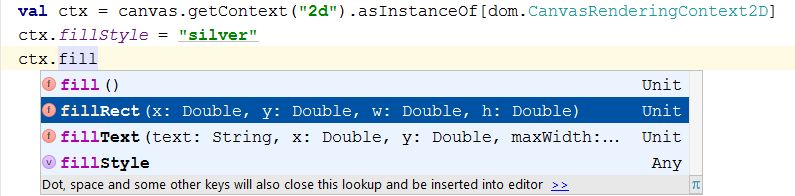
\includegraphics[width=1.0\textwidth]{typesafe-autocomplete}
    \caption{Intelligente Auto-Vervollständigung in IntelliJ.}
    \label{fig:typesafe-autocomplete}
\end{figure}


	-> Contra (?) bzw. Achtung ->  man muss durch Disziplin selbst darauf achten, dass man js.Dynamic vermeidet und ggf. castet, ist aber selten nötig (-> andere Beispiele???)




\subsection{Workbench-Plugin <- AUSLAGERN}

\TODO{EIGENES MINI-KAPITEL}

Damit das Workbench-Plugin von sbt auch geladen wird, muss es in der \code{plugins.sbt} hinzugefügt werden:

\begin{lstlisting}[style=snippet]
addSbtPlugin("com.lihaoyi" % "workbench" % "0.2.3")
\end{lstlisting}

In der build.sbt müssen folgende Einträge hinzugefügt werden:
\begin{lstlisting}[style=snippet]
workbenchSettings

bootSnippet := "frenzy.CanvasApp().main();"

updateBrowsers <<= updateBrowsers.triggeredBy(fastOptJS in Compile)
\end{lstlisting}

Das \code{bootSnippet} legt fest, welcher JavaScript als Einsprungspunkt für das Neuladen verwendet werden soll. Manchmal genügt ein \code{updateBrowsers} nicht, für solche Fälle existiert das radikalere:

\begin{lstlisting}[style=snippet]
refreshBrowsers <<= refreshBrowsers.triggeredBy(fastOptJS in Compile)
\end{lstlisting}

Nun muss die Workbench noch in der Entwicklungsversion des \ac{HTML}-Dokuments eingebunden werden durch folgenden Code-Schnipsel:

\begin{lstlisting}[language=HTML5, style=snippet]
<script src="/workbench.js"></script>
\end{lstlisting}

Hierbei ist es wichtig, darauf zu achten, dass diese Zeile nach allen anderen JavaScript-Einbindungen ganz am Ende im \html{<body>} steht.

Beim Start von sbt wird nun automatisch das Workbench-Plugin geladen. Dieses startet einen lokalen Server für das Projektwurzelverzeichnis unter der Adresse \url{localhost/127.0.0.1:12345}. Dadurch ist mit der Eingabe der Adresse \url{http://localhost:12345/target/scala-2.11/classes/index-dev.html} im Browser die Scala.js-Anwendung erreichbar.

Zur flüssigen Entwicklung ist es am komfortabelsten, im kontinuierlichen Modus zu arbeiten. Dazu wird nun \code{\~fastOptJS} aufgerufen, wodurch jedes Speichern von Code-Änderungen einen Build triggert. Ist hierbei die Workbench gestartet, muss das Terminal während der Entwicklung seltener aufgesucht werden, denn selbst Ausgaben des Compilers werden nützlicherweise in der Browser-Konsole ausgegeben (siehe Abb. \ref{fig:workbench-in-action1} - \ref{fig:workbench-in-action4}).

\begin{figure}[!h]
    \centering
    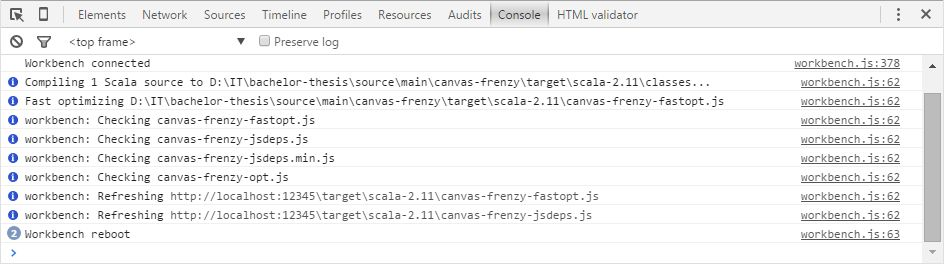
\includegraphics[width=1.0\textwidth]{workbench-in-action1}
    \caption{Ausgabe des Scala.js-Compilers in der Browser-Konsole.}
    \label{fig:workbench-in-action1}
\end{figure}

\begin{figure}[!h]
    \centering
    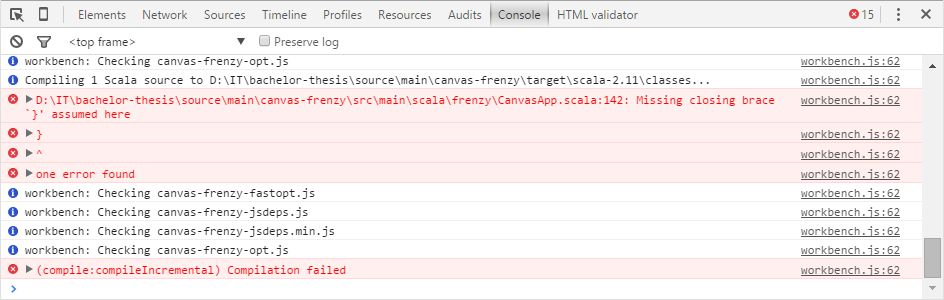
\includegraphics[width=1.0\textwidth]{workbench-in-action2}
    \caption{Fehlerausgabe des Scala.js-Compilers in der Browser-Konsole.}
    \label{fig:workbench-in-action2}
\end{figure}

Das Workbench-Plugin funktioniert nicht immer ganz zuverlässig, und manchmal muss das Browserfenster per Hand neu geladen werden. Alles in allem ist es aber ein sehr hilfreiches Entwicklungswerkzeug für ein flüssigeres Arbeiten.



% % % % % % % % % % % % % % % % % % % % % % % % % % % % % % % %
\section{Ajax}

\TODO{Projekt: sjs-currency-converter}

Die Kommunikation mit Objekten außerhalb des Web-Clients, zum Beispiel mit Webservices, ist ein wichtiger Bestandteil der meisten interaktiven Web-Anwendungen. Dazu wird standardmäßig eine als \emph{Ajax} bezeichnete Technik verwendet. Hierbei werden aus der Web-Anwendung heraus über das \ac{HTTP} Daten von einem Server angefragt, um auf Grundlage der Antwort Teile der \ac{HTML}-Seite zu aktualisieren. \cite[S.~491]{flanagan2011.JDG} Diese Aufrufe geschehen asynchron, das heißt die Seite blockiert nicht, sondern bleibt weiter bedienbar, während auf die Antwort vom Server gewartet wird. Diese Standardtechnik und der Umgang mit Asynchronität sollte mit Scala.js erprobt werden.


\MyMiniSec{Kurzbeschreibung des Währungsumrechners}

Beispielhaft wurde ein Währungsumrechner umgesetzt, der dem Benutzer die Eingabe des Betrags und die Auswahl von Quell- und Zielwährung per Auswahlliste anbietet, und auf Knopfdruck oder Betätigung der Entertaste hin die Umrechnung auf der Basis tagesaktueller Kurse durchführt. Beträge werden bis auf vier Nachkommastellen hin genau dargestellt. Die Eingabe ist fehlertolerant gegenüber ungültigen Beträgen. Als kleiner Komfort kann der Betrag mit der Escape-Taste auf 1.0000 zurückgesetzt werden. \TODOi{>>> bessere Bildqualität... >>>}

\begin{figure}[!h]
    \centering
    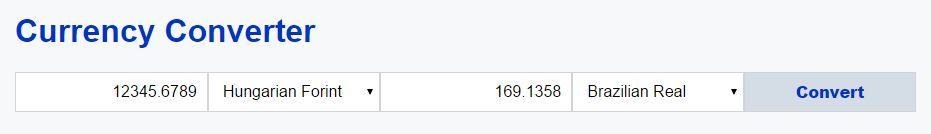
\includegraphics[width=1.0\textwidth]{currency-converter/currency-converter}
    \caption{Der Währungsumrechner.}
    \label{fig:converter}
\end{figure}

\MyMiniSec{Code-Qualität: Lesbarkeit, Wiederverwendbarkeit, Redundanzfreiheit}

Das Umrechnungsformular lässt sich mit ScalaTags sehr übersichtlich und deklarativ schreiben. Es werden zwei nahezu identische Währungsauswahllisten benötigt, mit einem Unterschied: Der Auswahlwert soll einmal als Quell-, das andere Mal als Zielwährung behandelt werden. Es wird eine Methode \scala{setupCurrencySelect} formuliert, die Auswahllisten erzeugt (Listing \ref{code:setupCurrencySelect}).

\begin{lstlisting}[language=Scala, caption={Eine Methode zur Erzeugung eines \html{<select>}-Elements.}, label={code:setupCurrencySelect}]
def setupCurrencySelect(theId: String,
                        updateConverter: String => Unit,
                        defaultOption: String = "EUR"): html.Select = {
  val sel = select(
    id:=theId,
    for ((code, name) <- Converter.currencies.toSeq) yield option(
      id:=s"$theId-opt-${code.toLowerCase}",
      value:=code, name
    )
  ).render
  sel.onchange = (e: dom.Event) => updateConverter(sel.value)
  sel.value = defaultOption
  sel
}
\end{lstlisting}

Dieser Methode muss eine Funktion \scala{String => Unit} übergeben werden, die den Auswahlwert entgegennimmt, so dass der Umrechner passend aktualisiert werden kann. Die Liste der möglichen \html{<option>}s lässt sich prägnant mithilfe einer \scala{for}-Comprehension ausdrücken. Das Auswahllisten-Element, bei dem es sich um ein \scala{TypedTag[html.Select]} handelt, muss durch Aufruf der Methode \scala{render} in den Fassadentyp \scala{html.Select} der Scala-js-dom-Bibliothek umgewandelt werden. Dadurch ist voller, typsicherer Zugriff auf die Methoden und Attribute möglich, die in der \ac{DOM}-\ac{API} spezifiziert sind. Ein \scala{onchange}-Handler ließe sich eigentlich auch innerhalb des \scala{select()}-Tags schreiben, allerdings ließe sich so nicht auf das \scala{value}-Attribut zugreifen.

Nach dieser Vorbereitung kann das Umrechnungsformular sehr übersichtlich und deklarativ geschrieben werden (Listing \ref{code:currency-converter-gui}).

\begin{lstlisting}[language=Scala, caption={Deklaration eines Formulars zur Währungsumrechnung mit ScalaTags.}, label={code:currency-converter-gui}]
container.appendChild(
  div(
    h1("Currency Converter"),
    form(
      onsubmit:={ (evt: dom.Event) => evt.preventDefault() },
      inputAmount,
      setupCurrencySelect("sel-src-curr", c => converter = converter.copy(srcCurr = c)),
      outputAmount,
      setupCurrencySelect("sel-dst-curr", c => converter = converter.copy(dstCurr = c)),
      button(
        cls:="input-btn",
        "Convert",
        onclick:={ () => updateDstAmount() }
      )
    )
  ).render
)
\end{lstlisting}

Die Felder für Eingabe (\scala{inputAmount}) und Ergebnis (\scala{outputAmount}) wurden zuvor definiert und mit \scala{.render} umgewandelt, damit sie im Programm referenziert werden können. Das hat den Vorteil, dass es so nicht nötig ist, den Umweg über \scala{document.getElementById()} jQuery-Selektoren zu gehen.

Eine Schwierigkeit im Umgang mit ScalaTags besteht allerdings darin, dass es manchmal schwierig ist, die richtigen Importe vorzunehmen. Häufig ist der Import von \scala{JsDom.all\_} ausreichend, allerdings werden hierdurch viele Namen in den Namensraum gebracht, was zu Konflikten führen kann, wenn man seltener benutzte Tags aus einem anderen Bundle verwenden möchte. Hier kann es auch helfen Aliase für schon importierte Namen einzuführen.


\MyMiniSec{Ajax mit XMLHttpRequest}

Für die Umrechnung wurde eine Klasse \scala{Converter} definiert. Als Quelle für die Umrechnungskurse sollte die Yahoo! Finance \ac{API}\footnote{\url{https://code.google.com/p/yahoo-finance-managed/wiki/YQLAPI}} genutzt werden, die auf \ac{HTTP}-Anfrage hin Ergebnisse im JSON-Format\footnote{\ac{JSON}, ein kompaktes Format zum Datenaustausch.} liefert. Anfragen werden in einer Query-Language formuliert. Die Anfrage:

\begin{lstlisting}[aboveskip=0pt, style=snippet]
http://query.yahooapis.com/v1/public/yql?q=select * from yahoo.finance.xchange where pair in ('EURUSD')&format=json&env=store://datatables.org/alltableswithkeys
\end{lstlisting}

liefert als Resultat das \ac{JSON}:

\begin{lstlisting}[language=JavaScript, style=snippet]
{
  "query": {
    "count": 1,
    "created": "2015-10-25T12:58:36Z",
    "lang": "de",
    "results": {
      "rate": {
          "id": "EURUSD",
          "Name": "EUR/USD",
          "Rate": "1.1018",
          "Date": "10/24/2015",
          "Time": "11:55am",
          "Ask": "1.1022",
          "Bid": "1.1013"
      }
    }
  }
}
\end{lstlisting}

Um \ac{HTTP}-Requests mit Scala.js zu realisieren gibt es verschiedene Möglichkeiten \cite[\#UsingWebServices]{haoyi.HOS}. Dank Scala-js-dom kann das \code{XMLHttpRequest}-Objekt\footnote{Eine ursprünglich von Microsoft entwickelte \ac{API} zur Client-Server-Kommunikation, die von den großen Browserherstellern Mozilla, Apple, and Google unterstützt und gegenwärtig vom \ac{W3C} standardisiert wird. \cite{mdn.XHR}} ganz ähnlich wie mit reinem Java-Script verwendet werden (allerdings typsicher).

\begin{lstlisting}[language=Scala, caption={HTTP-Aufruf mit XMLHttpRequest.}]
val xhr = new dom.XMLHttpRequest()
xhr.open("GET", url)
xhr.onload = (e: dom.Event) => {
  if (xhr.status == 200) {
    handleXhrResponse(xhr)
  }
}
xhr.send()
\end{lstlisting}

Der \scala{onload}-Handler wird als anonyme Funktion übergeben, semantisch ganz analog zu JavaScript:

\begin{lstlisting}[language=JavaScript, style=snippet]
xhr.onload = function(e) { /* ... */ } // JavaScript
\end{lstlisting}


\MyMiniSec{Ajax mit Futures und Async, Deserialisierung von JSONs}

\code{XMLHttpRequest} verlangt relativ viel Handarbeit, bietet aber dafür einen sehr direkten Zugriff auf das \ac{HTTP}-Protokoll. Für viele Anwendungsfälle ist das jedoch gar nicht nötig. Damit diese prägnanter geschrieben werden können, bietet Scala-js-dom Bequemlichkeitsmethoden für die gebräuchlichsten \ac{HTTP}-Methoden (GET, POST, PUT und DELETE). Diese Methoden geben eine \scala{Future[dom.XMLHttpRequest]}\footnote{Futures in Scala: \url{http://docs.scala-lang.org/overviews/core/futures.html}} zurück. Damit Futures und Promises in Scala.js verwendet werden können, wird ein Ausführungskontext benötigt \cite[\#Extensions]{scala-js-dom.DOC}. Zwei zusätzliche Importe sind nötig, der GET-Aufruf schrumpft dafür auf einen Einzeiler:

\begin{lstlisting}[language=Scala, caption={Futures-basierter HTTP-Aufruf mit Scala.js-Bequemlichkeitsmethode.}]
import org.scalajs.dom.ext.Ajax
import scala.scalajs.concurrent.JSExecutionContext.Implicits.runNow

Ajax.get(url).onSuccess{ case xhr => handleXhrResponse(xhr) }
\end{lstlisting}

Mit diesem Wissen wurde eine \scala{Converter}-Klasse definiert, die \emph{immutable} ist. Für jedes Währungspaar soll ein neue Instanz erzeugt werden.

\begin{lstlisting}[language=Scala, caption={Der Währungsumrechner.}]
case class Converter(
  srcCurr: String = "EUR",
  dstCurr: String = "EUR"
) {
  def convert(srcAmount: Double): Future[Double] = async{
    srcAmount * await{ rate }
  }

  private def url = "http://query.yahooapis.com/v1/public/yql?q=select * from yahoo.finance.xchange where pair in ('" + srcCurr + dstCurr + "')&format=json&env=store://datatables.org/alltableswithkeys"

  private lazy val rate: Future[Double] = Ajax.get(url).map{ case xhr =>
    val json: js.Dynamic = js.JSON.parse(xhr.responseText)
    json.query.results.rate.Rate.toString.toDouble
  }
}
\end{lstlisting}

Durch den Aufruf von \scala{JSON.parse} wird der Antworttext deserialisiert. Dabei erhält man ein dynamisch getyptes Objekt. Hier muss besonders sorgfältig vorgegangen werden, denn der Compiler schützt einen dabei nicht vor Tippfehlern. Die Rate muss zur sinnvollen Verwendung zuerst in einen String, und dieser dann in einen \scala{Double}-Wert umgewandelt werden.

Die Methode \scala{convert} soll den Ergebnisbetrag als \scala{Future[Double]} zurückzuliefern. Hierzu werden \scala{srcAmount: Double} und \scala{rate: Future[Double]} benötigt. Um die Handhabung von Futures zu vereinfachen wird hier ein \scala{async}-Block verwendet. Futures können, wenn sie in ein \scala{await} geschachtelt sind, innerhalb eines \scala{async}-Blocks behandelt werden, als wäre ihr Ergebnis schon bekannt. Auf diese Weise lässt sich die Intention sehr klar ausdrücken: Der Quellbetrag soll mit dem Umrechnungskurs multipliziert werden.

Nun kann eine Methode geschrieben werden, die auf Knopfdruck eine \ac{HTTP}-Anfrage beim Webservice stellt und beim Eintreffen der Antwort dafür sorgt, dass der umgerechnete Betrag auf der Webseite angezeigt wird.

\begin{lstlisting}[language=Scala, style=snippet]
def updateDstAmount(): Unit = converter.convert(srcAmount).onSuccess{
  case dstAmount => outputAmount.textContent = format(dstAmount)
}
\end{lstlisting}

Es lässt sich festhalten, dass Ajax-Aufrufe mit Scala.js lesbar und prägnant formuliert werden können.


\MyMiniSec{Formatierung von Zahlen}

Zahlenwerte müssen zur einheitlichen Ausgabe in Scala.js praktisch immer nötig passend formatiert werden (siehe Abschnitt \ref{subsec:sjs-primitives}). Um einen Wert \scala{val foo = 1.234f} auf vier Nachkommastellen zu beschränken, kann zum Beispiel \scala{f\"\$foo\%.4f\"} oder auch \linebreak\mbox{\scala{\"\%.4f\".format(foo)}} oder \scala{foo.formatted(\"\%.4f\")} verwendet werden. Die direkte Verwendung der Java-Methode \scala{String.format()} funktioniert nicht. Eine weiter Möglichkeit wäre aber, nach Import von \scala{scala.scalajs.js.JSNumberOps.\_} die native JavaScript-Methoden \scala{foo.toFixed(4)} zu verwenden.


\MyMiniSec{Dokumentation}

Die Dokumentation der verwendeten Librarys Scala-js-dom, ScalaTags, und Scala-Async sowie das E-Book \cite[\#UsingWebServices]{haoyi.HOS} waren bei der Erstellung der Anwendung äußerst aufschlussreich und boten wichtige Orientierungshilfe. Die \ac{API}-Dokumenatation im Sourcecode ist hingegen noch sehr wortkarg.



% % % % % % % % % % % % % % % % % % % % % % % % % % % % % % % %
%\section{js-interop -> playground(?) (3)}
%
%\subsection{Ziel der Untersuchung}
%\subsection{Untersuchungskriterien}
%\subsection{Kurzbeschreibung des Beispielprogramms}
%\subsection{Ergebnisse der Untersuchung und Bewertung}
%\subsection{Schwierigkeiten}
%\subsection{Erfolge}
%\subsection{Bewertung: differenziert oder boolsch mit Begründung; Fazit aus Schwierigkeiten und Erfolgen}

% % % % % % % % % % % % % % % % % % % % % % % % % % % % % % % %
\section{Eine Cross-kompilierende Library}

\TODO{Projekte: sjs-crosscompiling-statistics-lib, js-port-of-statistics-lib, benchmark-statistics-libs}

Die Wiederverwendbarkeit von Code für Client \emph{und} Server ist ein wünschenswertes Ziel. Hier sollte anhand der Implementierung einer kleinen cross-kompilierenden Library erprobt werden, wie das mit Scala.js möglich ist. Außerdem sollte durch Tests die Korrektheit der Bibliothek sichergestellt werden. 
Außerdem sollte die implementierten Scala.js-Library in natives HTML/JavaScript eingebunden werden, um auch die Interoperabilität zu erproben. Schließlich sollte eine Portierung nach JavaScript vorgenommen werden um einerseits einen Vergleich des Codes aber vor allem auch einen Leistungsvergleich zwischen Scala.js und nativem JavaScript vornehmen zu können.

%BILD -> \cite[Folie 52, Min. ???]{doeraene2015.SSP} % -->  Doeraene2015-Scalajs-p52.jpg


\MyMiniSec{Kurzbeschreibung der Statistik-Library}

Es wurde eine kleine Statistik-Library implementiert. Diese bietet die zur Auswertung einer Zahlenfolge die 
vier Funktionen: Mittelwert, Median, Varianz und Standardabweichung.

\MyMiniSec{Kurzbeschreibung der Statistik-GUI}

Es eine einfache GUI mit \ac{HTML}, \ac{CSS} und nativem JavaScript implementiert, welche die Statistik-Library verwendet
(siehe Abb. \ref{fig:stat-lib-gui}). In ein Eingabefeld können Zahlen, getrennt durch Komma oder Whitespace eingetragen werden. Dabei ist die Eingabe fehlertolerant gegenüber von eingestreuten nicht-numerischen Zeichen. Über eine Auswahlliste kann die gewünschte Berechnung ausgewählt werden. Durch Betätigen der Entertaste im Eingabefeld wird die Zahlenfolge ausgewertet und das Ergebnis angezeigt.

\begin{figure}[!h]
    \centering
    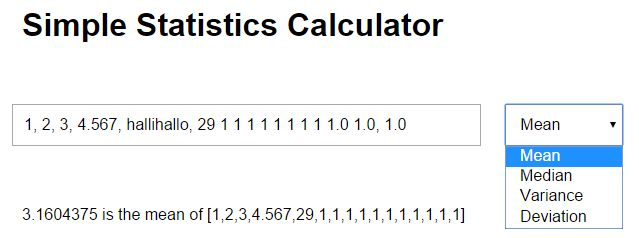
\includegraphics[width=0.75\textwidth, frame]{statistics-lib/statistics-gui}
    \caption{Einfache GUI der Statistik-Bibliothek im Browser.}
    \label{fig:stat-lib-gui}
\end{figure}


\MyMiniSec{Cross-Projekt}

Das cross-kompilierende Projekt hat eine Struktur wie in Listing \ref{code:cross-project-struct} dargestellt. Die Struktur orientiert sich an den Hinweisen der Scala.js-Dokumenation \cite{scalajs.CBP}, wo auch die nötige Konfiguration der \code{build.sbt} beschrieben ist.

\begin{lstlisting}[language=scala, caption={Struktur der cross-kompilierenden Scala.js-Library}, label={code:cross-project-struct}]
library
 +- js
 |   +-src
 |      +- main
 |      +- test
 +- jvm
 |   +-src
 |      +- main
 |      +- test
 +- shared
     +-src
        +- main
        +- test
\end{lstlisting}

Die Funktionalität wurde im \code{shared}-Projekt implementiert. In \code{js} und \code{jvm} existieren jeweils plattformspezifische Fassaden, die Methodenaufrufe an die geteilte Implementierung delegieren.


\MyMiniSec{JavaScript-Interoperabilität}

Die kompilierten JavaScript-Artefakte des Cross-Projekts finden sich im Verzeichnis \code{library/js/target/}.

Es gibt eine JavaScript-spezifische Fassade mit den zum Export nötigen Annotationen; auch wird hier der \js{js.Array}-Typ verwendet:

\begin{lstlisting}[language=Scala, style=snippet]
package platform

@JSExport
object StatLib {
  @JSExport def mean(seq: js.Array[Double]): Double = statistics.Statistics.mean(seq)
  ...
}
\end{lstlisting}

Die kompilierte Library kann wie gewohnt in ein \ac{HTML}-Dokument eingebunden werden:

\begin{lstlisting}[language=HTML5, style=snippet]
<script src="../statistics-lib-js-opt.js"></script>
<script src="Util.js"></script>
\end{lstlisting}

In der JavaScript-Datei \js{Util.js} mit der Oberflächenlogik kann die Library nun verwendet werden:

\begin{lstlisting}[language=JavaScript, style=snippet]
var stat = platform.StatLib();
stat.deviation([1, 2, 3])
\end{lstlisting}


\MyMiniSec{Tests}

Für die cross-kompilierende Library wird durch drei äquivalente Test-Suiten mit uTest in allen drei Unterprojekten das gleichwertige Funktionieren auf beiden Plattformen geprüft. Tests können für beide Plattformen, oder auch nur gezielt für JavaScript oder \ac{JVM} ausgeführt werden.

Für die JavaScript-Portierung wurden entsprechende 
Tests für das JavaScript-Test-Werkzeug Jasmine erstellt.


\MyMiniSec{Code-Qualität}

Die Funktionen lassen sich mit Scala sehr knapp formulieren.

Im Vergleich fiel bei der Portierung in natives JavaScript fiel sofort auf, dass mehr Hilfs-Methoden selbst geschrieben werden müssen. Um performante Funktionen zu erhalten, konnte in nativem JavaScript nicht auf die funktionalen Methoden \js{Array}-Methoden wie \js{map} zurückgegriffen werden, denn diese sind im Vergleich mit einer iterativen Implementierung etwa zehnmal langsamer, wie ein separater Benchmark-Test ergab.


\MyMiniSec{Vergleichender Benchmark}

Die Ergebnisse des vergleichenden Benchmarks der Statistik-Funktionen zeigen Abbildung \TODOi{6.9(??) und Tabelle 6.4 (??))}. Dabei sind die verschiedenen Funktionen an ihrem Suffix zu unterscheiden: \code{js} für JavaScript und \code{sjs} für Scala.js. Die Maßeinheit sind Operationen pro Sekunde.

Demnach sind die Scala.js-Implementierungen ist etwa 9 \% \TODOi{ CHECK AGAIN } langsamer als natives JavaScript (wenn in JavaScript auf Funktionen höherer Ordnung verzichtet wird).

Damit sind beide Implementierungen doch recht nahe beieinander. Die etwas geringere Leistungsfähigkeit sollte nur bei äußerst leistungshungrigen Anwendungen ins Gewicht fallen.

Durch den Einsatz von Scala.js gewinnt man hingegen eine plattformübergreifende Implementierung, die außerdem den Vorteil hat, dass funktional programmiert werden kann.

Das führt deshalb nicht zu einem heftigen Leistungsabfall, weil der Optimierer die Funktionsaufrufe ...

\begin{figure}[!h]
	\centering
	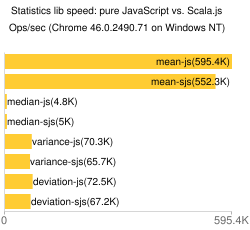
\includegraphics[width=0.35\textwidth]{statistics-lib/benchmark-statistics-lib-chart}
	\qquad
	\qquad
	\begin{tabular}[b]{|l|r|}
		\hline \textbf{Test} & \textbf{Ops/sec} \\ 
		\hline mean-js       & 595399 \\ 
		\hline mean-sjs      & 552250 \\ 
		\hline median-js     & 4839 \\ 
		\hline median-sjs    & 5049 \\ 
		\hline variance-js   & 70267 \\ 
		\hline variance-sjs  & 65650 \\ 
		\hline deviation-js  & 72506 \\ 
		\hline deviation-sjs & 67156 \\ 
		\hline 
	\end{tabular}
	\captionlistentry[table]{Benchmark der Statistik-Bibliothek.}
	\captionsetup{labelformat=andtable}
	\caption{Benchmark der Statistik-Bibliothek.}
\end{figure}







% % % % % % % % % % % % % % % % % % % % % % % % % % % % % % % %
\chapter{Fazit}\label{chap:conclusion}

 \section{Zusammenfassung der Ergebnisse}

Was war wirklich wichtig bei der Arbeit?
- Überblick gewinnen
- Nützlichkeit und Einsetzbarkeit praktisch erproben
Wie sieht das Ergebnis aus?
- siehe alles hier drunter ...
Wie schätzen Sie das Ergebnis ein?
- 
Gab es Randbedingungen, Ereignisse, die die Arbeit wesentlich beeinflußt haben?
- Scala lernen, speziell abgefahrenes wie implicits
- gleichzeitig DOM-API
- Unerfahrenheit
- junges Projekt
	- noch keine gedruckten Quellen
	- Entwicklung im Wandel
Gibt es noch offene Probleme?
- benchmark von sjs läuft nicht mit aktueller version
- siehe unten ...
Wie könnten diese vermutlich gelöst werden?
- siehe unten ...





\TODO{- Scala.js bringt Scala (bisher auf Basis der jvm -> %\ac{JVM}
) auf die Client-Seite:}


Dependencys bequem gemanagt mit sbt, wenig muss in die html eingetragen werden, das meißte zentral in der build.sbt


   Korrektheit \\
	-> doeraene TDI S.7, links \\
   Performance \\
	--> doeraene TDI S. 7, oben rechts \\
	(-> eigenes Micro-Benchmark -> Bsp.) \\
>> Nützlichkeit \\
	- getypter \ac{DOM} \\
	- getypte Fassaden für jQuery und Libs \\
	- bei Bedarf: js.Dynamic \\

Die vorliegende Arbeit ... \\
- Überblick über Entwicklung von Weboberflächen mit Scala.js \\
- Eignung aus Anwendersicht ... \\
- Eignung aus Entwicklersicht ... \\
- Vorteile ... \\
	- vollständiger Scala-Support \\
	- umfassende JS-Interop \\
	- sbt-Integration \\
	- Typsicherheit \\
		- weniger Fehler \\
		- \ac{IDE}-Support! \\
	- Source Maps zum besseren Debugging \\
- Nachteile ... \\
	- noch etwas große Kompilate \\
	- Doku momentan noch etwas (!) unübersichtlich und im Wandel, nicht ganz vollständig \\
		- ein Beispiel hier: \url{http://www.scala-js.org/doc/cookbook/} \\
		Dokumentation: \\
		- offizielle Referenzseite \\
		- \ac{API}-Doku - vollständig (?) aber knapp \\
		- Tutorial \\
		- Hands-on Scala \\
		- Scala-Js-Fiddle  -->  \url{http://www.scala-js-fiddle.com/} \\
		
		API nur sporadisch ausführlicher beschrieben

Pro Scala.js: \\
    - direkt mit dem \ac{DOM} arbeiten, aber getypt \\
    - zwischen Client/Server geteilt: Konstanten, Algorithmen, Datenstrukturen, Librarys \\
    - Typsicherheit \\
    - Interface zwischen Client/Server \\
    - Scala-Programmierer können ohne die Sprache zu wechseln fürs Web programmieren \\
    - inkrementelle Kompilation, DCE (Dead code elemination) \\
Contra Scala.js: \\
    - small Community \\
    - kleines Entwicklerteam, keine Unterstützung durch ein größere Firma \\
    - langsamer Scala-Compiler \\
    - große Bibliothek --> relativ große Kompilate \\





>> was spricht für Scala.js? \\
    nach nicht-repräsentativer Umfrage ( \\
      vgl.  -->  \url{http://www.scala-lang.org/news/2015/02/05/scala-js-no-longer-experimental.html} \\
      Diskussion hier  -->  \url{https://groups.google.com/forum/#!topic/scala-js/_1Sfb5Nj08w} \\
    ): \\
    - geteilter Code zwischen Client und Server, eine Sprache für die gesamte Anwendung, z.B. für Validierungs-Logik, aber auch \\ Wiederverwendbarkeit von Code (wenn keine Plattformspezifika direkt verwendet werden) \\
    \cite{doeraene2013.CSJ} \\
    - starke Typisierung, auch für JavaScript-Librarys \\
    - Tooling: \ac{IDE}-Support, sbt-Integration, Dependency-Management, Unit-Tests, Stacktraces und Source Maps, kross-compilierende Projekte \\
    - Portababilität: Scala auf JavaScript-basierten Plattformen \\

  kompletter Scala-Support \\
  
  schnelle Ints: \\
  - Int-Operationen werden durch bitweise Veroderung umgesetzt (z.B. Scala.js: a + b -> JS: (a + b) | 0) \\
  - JS VMs verwenden intern int32 als Optimierung für bitweise Operationen \\
  -> schneller\cite{doeraene2015.SSP} \\


  schneller Dev-cycle, optim. Prod.code \\
  
  Scala im Browser!!! \\
  
  
was fehlt? \\
  (- checked Exceptions???) \\
  (- Regex???) \\
  - Unterstützung von Laufzeit-Reflection \\

Schwächen \\
  - relativ große Dateien \\
  (- Debugging schwieriger???) \\
  - Support für einige Librarys \\
  - Performance \\
  
Unbequemlichkeiten \\
  - Auslieferung von Produktionscode noch etwas mühsam: kompiliert nach \\
\begin{lstlisting}
target/
  +- scala-2.11/
  +- [...]-opt.js
  +- [...]-jsdeps.min.js
  +- classes/
      +- index.html
      +- [...].css
\end{lstlisting}
  - muss per Hand extrahiert werden
  - wenn andere Ordnerstruktur gewünscht ist, z.B.:
\begin{lstlisting}
webapp/
 +- js/
 |   +- [...]-opt.js
 |   +- [...]-jsdeps.min.js
 +- css/
 |   +- [...].css
 +- index.html
\end{lstlisting}
  ... dann müssen die Pfade in der index.html entsprechend geändert werden \\
  -> Lösung wären hier entsprechende Export-Skripte; bzw. denkbar, dass in Zukunft ein entsprechendes Tool oder sbt-Plugin (?) angeboten wird \\



großes Potential \\
	besonders weil: eine Sprache für Client und Server \\
		Wiederverwendbarkeit von Code \\
		nur in einer Sprache denken, nicht eine weitere lernen \\
	typbedingte Laufzeitfehler auch für Client-Seite (JavaScript) ausgeschlossen sind \\
	mit Templating-Library auch \ac{HTML}-Tags typsicher macht \\
	
Doku noch im Wandel, stellenweise ("`tiefer drin"') noch etwas sparsam erklärt, zeitweise und sporadisch nicht mit den neuesten Änderungen synchron (/nicht auf dem aktuellsten Stand), aber im Großen und Ganzen ziemlich gut, erlaubt recht tiefen Einblick \\

vor allem für Entwickler und Projekte die schon mit Scala arbeiten sehr interessant \\

Erfolg hängt sicher auch am Erfolg der Sprache Scala \\
dafür, dass noch sehr jung, schon sehr gut entwickelt und anscheinend stabil \\




Hürden \\

- speziellere Konfiguration, besonders \\
  - für Cross-Projekte \\
  - vermutlich, wenn Vorgaben für die zu verwendenden Techniken bestehen \\

Chancen \\

- eine eindeutige, typsichere Schnittstelle zur Client-Server-Kommunikation \\





\section{Ausblick}

Nach zweieinhalb Jahren der Entwicklung hat Scala.js inzwischen einen stabilen Stand erreicht. Das Projekt wird neben Hauptenwickler sind Sébastien Doeraene und Tobias Schlatter (ebenfalls ein Mitarbeiter des \ac{EPFL}) von mittlerweile weiteren 33 beitragende Entwicklern vorangetrieben. Das Projekt ist auf GitHub\footnote{\url{https://github.com/scala-js/scala-js}} beheimatet. Seit Juni 2014 werden alle Release-Ankündigungen\footnote{\url{http://www.scala-js.org/archive.html}} auf der Website des Projekts archiviert. Neue Releases wurden im Verlauf des letzten Jahres etwa monatlich herausgebracht.

Eine interessante Verbesserung, die Ende August dieses Jahres mit Version 0.6.5\footnote{\url{http://www.scala-js.org/news/2015/08/31/announcing-scalajs-0.6.5/}} hinzugekommen ist, erlaubt es Scala.js-definierte JavaScript-Klassen mit JavaScript-Semantik zu schreiben, welche auch von JavaScript-Klassen erben können. Längerfristig geplante Weiterentwicklungen sind neben zusätzlichen Performance-Verbesserungen die volle Unterstützung von Laufzeit-Reflections \cite[S. 2]{doeraene2013.TDI}, ein Compiler im Browser \cite[Folie 39, Min. 39]{doeraene2014.WHB} und vollwertige Akka-Aktoren \cite[Folie 39, Min. 39]{doeraene2014.WHB}.

Viele Librarys, die Scala.js unterstützen befinden sich momentan noch in einem frühen Stadium, und so ist die Frage, ob Scala.js sich für den professionellen Einsatz eignet auch abhängig davon, wie sich das gesamte Ökosystem stabilisiert und ob es weiter so schnell wächst. Doch stehen die Chancen gut, angesichts der Erweiterungen befördernden Spracheigenschaften von Scala einerseits, und einer kleinen, aber enthusiastischen Scala.js-Community andererseits. Interessant für interaktive Weboberflächen könnten hier etwa die reaktiven Scala.Rx und Monifu oder auch die Anbindungen von UI-Frameworks wie AngularJS oder React sein.

Die Bereitschaft von Frontend-Entwicklern, welche mehrheitlich nicht mit Scala vertraut sein dürften, auf eine andere Sprache umzusteigen muss mindestens bezweifelt werden, ist dies doch mit einem recht hohen Lernaufwand verbunden. Ein Aufwand der sich allerdings sehr lohnen würde: für die Qualität der entwickelten Software, für die längerfristige zu erwartende Produktivität und für die Freude an der eigenen Arbeit. Und so wird der Erfolg von Scala.js sehr stark vom Erfolg der Sprache Scala abhängen.


%Blick über den Tellerrand:  anderer vielversprechender Ansatz: Elm -> url -> %http://elm-lang.org/
%- FRP (Functional Reactive Programming) Sprache um deklarativ UIs für den Browser zu schreiben, statisch typisiert \\
%- kompiliert nach \ac{HTML}, CSS und JavaScript \\
%- hat \ac{REPL}, package manager, debugger \\
%- librarys \\
%- Alternative zu Scala.js? - kein Scala, nur Client... \\








% % % % % % % % % % % % % % % % % % % % % % % % % % % % % % % %

% ANHANG ERSTELLEN
%\appendix
%\chapter{Quellcodeauszüge usw.}
%
%\section{Beispielcode}
%
%Ein kleines JavaScript-Codeschnipsel könnte man \lstinline[language=JavaScript, style=inline]!function(x) { return 2 + x; }! inline schreiben. Und ein kleines Scala-Codeschnipsel könnte man \lstinline[language=Scala, style=inline]|def foo(): Unit = println("bar")| inline schreiben.
%
%
%\begin{lstlisting}
%var sqr = function(x) { return x * x; }
%for (var i = 0; i < 10; i++) {
%  console.log(i, sqr(i));
%}
%\end{lstlisting}



% % % % % % % % % % % % % % % % % % % % % % % % % % % % % % % %
% % % % % % % % % % % % % % % % % % % % % % % % % % % % % % % %

% AKÜRZUNGSVERZEICHNIS ERSTELLEN
\clearpage
\markboth{Abkürzungsverzeichnis}{Abkürzungsverzeichnis}
\chapter*{Abkürzungsverzeichnis}
\addcontentsline{toc}{chapter}{Abkürzungsverzeichnis}
\begin{acronym}[HTML] % längste Abkürzung hier als Argument angeben
	\acro{API}{Application programming interface}
	\acro{CSS}{Cascading Style Sheets}
	\acro{DOM}{Document Object Model}
	\acro{DSL}{Domain-specific language}
	\acro{EPFL}{École polytechnique fédérale de Lausanne}
	\acro{HTML}{Hypertext Markup Language}
	\acro{HTTP}{Hypertext Transfer Protocol}
	\acro{IDE}{Integrated development environment}
	\acro{JSON}{JavaScript Object Notation}
	\acro{JVM}{Java Virtual Machine}
	\acro{REPL}{Read-eval-print loop}
	\acro{URL}{Uniform Resource Locator}
	\acro{W3C}{World Wide Web Consortium}
	\acro{XML}{Extensible Markup Language}
\end{acronym}

% ABBILDUNGSVERZEICHNIS ERSTELLEN
\listoffigures

% TABELLENVERZEICHNIS ERSTELLEN
\listoftables

% QUEELLCODEVERZEIHCHNIS ERSTELLEN
\lstlistoflistings

% LITERATURVERZEICHNIS ERSTELLEN
%\begin{thebibliography}{xxxxxxxxxxxxxxxxxxx}
%   \bibitem[BECK, ????]{BECK} Beck, Kent: Extreme Programming : Das Manifest, Addison-Wesley, ORT, JAHR. % TODO
%   \bibitem[ARIS, ????]{ARIS} Arisholm, Erik; Gallis, Hans; Dyb\aa , Tore; Sj\o berg, Dag I.K.: TITEL. In: IEEE Transcactions on Software
%    Engineering, Vol. 33, No. 2, Februar 2007.
%
%
%
%   \bibitem[GoF, 1994]{GoF1} Erich Gamma, Richard Helm, Ralph Johnson, John Vlissides: Design Patterns: Elements of reusable object oriented software Addison Wesley Publishing Company 1994, ISBN 0-201-63361-2
%   \bibitem[BMBF, 2003]{bmbf}"'IT-Ausstattung der allgemein bildenden und berufsbildenden Schulen in Deutschland"', http://www.schulen-ans-netz.de/neuemedien/fakten/dokus/it-ausstattung-2003.pdf, 10.03.2005
%\end{thebibliography}


% TODO: nocite entfernen, damit nur zitierte Literatur ins Verzeichnis kommt
%\nocite{*}


% Bibliographie mit bibtex
%\bibliographystyle{alphadin}
%\bibliography{biblio_scalajs}


% Bibliographie mit biblatex/biber
\printbibliography



%%%%%%%%%%%%%%%%%%%%%%%%%%%%%%%%%%%%%%%%%%%%
% END DOCUMENT // HIER HÖRT DER INHALT AUF
%%%%%%%%%%%%%%%%%%%%%%%%%%%%%%%%%%%%%%%%%%%%
\end{document}








